\documentclass[twoside]{article}

% Packages required by doxygen
\usepackage{calc}
\usepackage{doxygen}
\usepackage{graphicx}
\usepackage[utf8]{inputenc}
\usepackage{makeidx}
\usepackage{multicol}
\usepackage{multirow}
\usepackage{textcomp}
\usepackage[table]{xcolor}

% NLS support packages
\usepackage{polski}
\usepackage[T1]{fontenc}

% Font selection
\usepackage[T1]{fontenc}
\usepackage{mathptmx}
\usepackage[scaled=.90]{helvet}
\usepackage{courier}
\usepackage{amssymb}
\usepackage{sectsty}
\renewcommand{\familydefault}{\sfdefault}
\allsectionsfont{%
  \fontseries{bc}\selectfont%
  \color{darkgray}%
}
\renewcommand{\DoxyLabelFont}{%
  \fontseries{bc}\selectfont%
  \color{darkgray}%
}

% Page & text layout
\usepackage{geometry}
\geometry{%
  a4paper,%
  top=2.5cm,%
  bottom=2.5cm,%
  left=2.5cm,%
  right=2.5cm%
}
\tolerance=750
\hfuzz=15pt
\hbadness=750
\setlength{\emergencystretch}{15pt}
\setlength{\parindent}{0cm}
\setlength{\parskip}{0.2cm}
\makeatletter
\renewcommand{\paragraph}{%
  \@startsection{paragraph}{4}{0ex}{-1.0ex}{1.0ex}{%
    \normalfont\normalsize\bfseries\SS@parafont%
  }%
}
\renewcommand{\subparagraph}{%
  \@startsection{subparagraph}{5}{0ex}{-1.0ex}{1.0ex}{%
    \normalfont\normalsize\bfseries\SS@subparafont%
  }%
}
\makeatother

% Headers & footers
\usepackage{fancyhdr}
\pagestyle{fancyplain}
\fancyhead[LE]{\fancyplain{}{\bfseries\thepage}}
\fancyhead[CE]{\fancyplain{}{}}
\fancyhead[RE]{\fancyplain{}{\bfseries\leftmark}}
\fancyhead[LO]{\fancyplain{}{\bfseries\rightmark}}
\fancyhead[CO]{\fancyplain{}{}}
\fancyhead[RO]{\fancyplain{}{\bfseries\thepage}}
\fancyfoot[LE]{\fancyplain{}{}}
\fancyfoot[CE]{\fancyplain{}{}}
\fancyfoot[RE]{\fancyplain{}{\bfseries\scriptsize Wygenerowano Wt, 17 mar 2015 00\-:16\-:04 dla Laboratorium 2 programem Doxygen }}
\fancyfoot[LO]{\fancyplain{}{\bfseries\scriptsize Wygenerowano Wt, 17 mar 2015 00\-:16\-:04 dla Laboratorium 2 programem Doxygen }}
\fancyfoot[CO]{\fancyplain{}{}}
\fancyfoot[RO]{\fancyplain{}{}}
\renewcommand{\footrulewidth}{0.4pt}
\renewcommand{\sectionmark}[1]{%
  \markright{\thesection\ #1}%
}

% Indices & bibliography
\usepackage{natbib}
\usepackage[titles]{tocloft}
\setcounter{tocdepth}{3}
\setcounter{secnumdepth}{5}
\makeindex

% Hyperlinks (required, but should be loaded last)
\usepackage{ifpdf}
\ifpdf
  \usepackage[pdftex,pagebackref=true]{hyperref}
\else
  \usepackage[ps2pdf,pagebackref=true]{hyperref}
\fi
\hypersetup{%
  colorlinks=true,%
  linkcolor=blue,%
  citecolor=blue,%
  unicode%
}

% Custom commands
\newcommand{\clearemptydoublepage}{%
  \newpage{\pagestyle{empty}\cleardoublepage}%
}


%===== C O N T E N T S =====

\begin{document}

% Titlepage & ToC
\hypersetup{pageanchor=false}
\pagenumbering{roman}
\begin{titlepage}
\vspace*{7cm}
\begin{center}%
{\Large Laboratorium 2 \\[1ex]\large 0.\-2 }\\
\vspace*{1cm}
{\large Wygenerowano przez Doxygen 1.8.6}\\
\vspace*{0.5cm}
{\small Wt, 17 mar 2015 00:16:04}\\
\end{center}
\end{titlepage}
\tableofcontents
\pagenumbering{arabic}
\hypersetup{pageanchor=true}

%--- Begin generated contents ---
\section{Laboratorium 2}
\label{index}\hypertarget{index}{}Aplikacja umozliwia uzytkownikowi na przeprowadzenia algorytmu mnozenia\par
 przez dwa na dowolnej liczbie elementow.\par
\par


{\bfseries Najważniejsze cechy}\par
 Możliwość włączenia opcji benchmarkującej służącej do sprawdzenia\par
 ile czasu wykonywal sie dany algorytm lub seria tego samego algorytmu\par
\par


{\bfseries Argumenty wywołania} \begin{DoxyVerb}-n liczba       Ilość liczb do odczytania/przerobienia przez algorytm
-t liczba       Włącza opcje benchmarkującą dla seri powtorzen
-o tekst        Wprowadza nazwe pliku do zapisu
-i tekst        Wprowadza nazwe pliku do odczytu
-g              Generuje n liczb i zapisuje je do pliku (po wygenerowaniu konczy program)
\end{DoxyVerb}
 
\section{Indeks hierarchiczny}
\section{Hierarchia klas}
Ta lista dziedziczenia posortowana jest z grubsza, choć nie całkowicie, alfabetycznie\-:\begin{DoxyCompactList}
\item \contentsline{section}{Data\-Frame}{\pageref{class_data_frame}}{}
\begin{DoxyCompactList}
\item \contentsline{section}{My\-Benchmark}{\pageref{class_my_benchmark}}{}
\begin{DoxyCompactList}
\item \contentsline{section}{Multiply\-By\-Two}{\pageref{class_multiply_by_two}}{}
\end{DoxyCompactList}
\item \contentsline{section}{Number\-Generator}{\pageref{class_number_generator}}{}
\end{DoxyCompactList}
\end{DoxyCompactList}

\section{Indeks klas}
\subsection{Lista klas}
Tutaj znajdują się klasy, struktury, unie i interfejsy wraz z ich krótkimi opisami\-:\begin{DoxyCompactList}
\item\contentsline{section}{\hyperlink{class_data_frame}{Data\-Frame} }{\pageref{class_data_frame}}{}
\item\contentsline{section}{\hyperlink{class_multiply_by_two}{Multiply\-By\-Two} \\*Algorytm mnozy kazda liczbe razy 2 }{\pageref{class_multiply_by_two}}{}
\item\contentsline{section}{\hyperlink{class_my_benchmark}{My\-Benchmark} \\*Klasa bazowa/interface do testowania algorytmu }{\pageref{class_my_benchmark}}{}
\item\contentsline{section}{\hyperlink{class_my_list}{My\-List} \\*Lista dwukierunkowa }{\pageref{class_my_list}}{}
\item\contentsline{section}{\hyperlink{class_my_list_1_1_my_list_element}{My\-List\-::\-My\-List\-Element} \\*Klasa 'malych struktur' gdzie jest numer i wskaznik do nas elementu }{\pageref{class_my_list_1_1_my_list_element}}{}
\item\contentsline{section}{\hyperlink{class_my_queue}{My\-Queue} \\*Klasa reprezentuje kolejke }{\pageref{class_my_queue}}{}
\item\contentsline{section}{\hyperlink{class_my_stack}{My\-Stack} \\*Klasa reprezentuje stos }{\pageref{class_my_stack}}{}
\item\contentsline{section}{\hyperlink{class_number_generator}{Number\-Generator} \\*Klasa generujaca losowe liczby }{\pageref{class_number_generator}}{}
\end{DoxyCompactList}

\section{Indeks plików}
\section{Lista plików}
Tutaj znajduje się lista wszystkich plików z ich krótkimi opisami\-:\begin{DoxyCompactList}
\item\contentsline{section}{\hyperlink{dataframe_8cpp}{dataframe.\-cpp} }{\pageref{dataframe_8cpp}}{}
\item\contentsline{section}{\hyperlink{dataframe_8d}{dataframe.\-d} }{\pageref{dataframe_8d}}{}
\item\contentsline{section}{\hyperlink{dataframe_8h}{dataframe.\-h} }{\pageref{dataframe_8h}}{}
\item\contentsline{section}{\hyperlink{main_8cpp}{main.\-cpp} }{\pageref{main_8cpp}}{}
\item\contentsline{section}{\hyperlink{main_8d}{main.\-d} }{\pageref{main_8d}}{}
\item\contentsline{section}{\hyperlink{multiplybytwo_8cpp}{multiplybytwo.\-cpp} }{\pageref{multiplybytwo_8cpp}}{}
\item\contentsline{section}{\hyperlink{multiplybytwo_8d}{multiplybytwo.\-d} }{\pageref{multiplybytwo_8d}}{}
\item\contentsline{section}{\hyperlink{multiplybytwo_8h}{multiplybytwo.\-h} }{\pageref{multiplybytwo_8h}}{}
\item\contentsline{section}{\hyperlink{mybenchmark_8cpp}{mybenchmark.\-cpp} }{\pageref{mybenchmark_8cpp}}{}
\item\contentsline{section}{\hyperlink{mybenchmark_8d}{mybenchmark.\-d} }{\pageref{mybenchmark_8d}}{}
\item\contentsline{section}{\hyperlink{mybenchmark_8h}{mybenchmark.\-h} }{\pageref{mybenchmark_8h}}{}
\item\contentsline{section}{\hyperlink{numbergenerator_8h}{numbergenerator.\-h} }{\pageref{numbergenerator_8h}}{}
\end{DoxyCompactList}

\section{Dokumentacja klas}
\hypertarget{class_data_frame}{\subsection{Dokumentacja klasy Data\-Frame}
\label{class_data_frame}\index{Data\-Frame@{Data\-Frame}}
}


{\ttfamily \#include $<$dataframe.\-h$>$}

Diagram dziedziczenia dla Data\-Frame\begin{figure}[H]
\begin{center}
\leavevmode
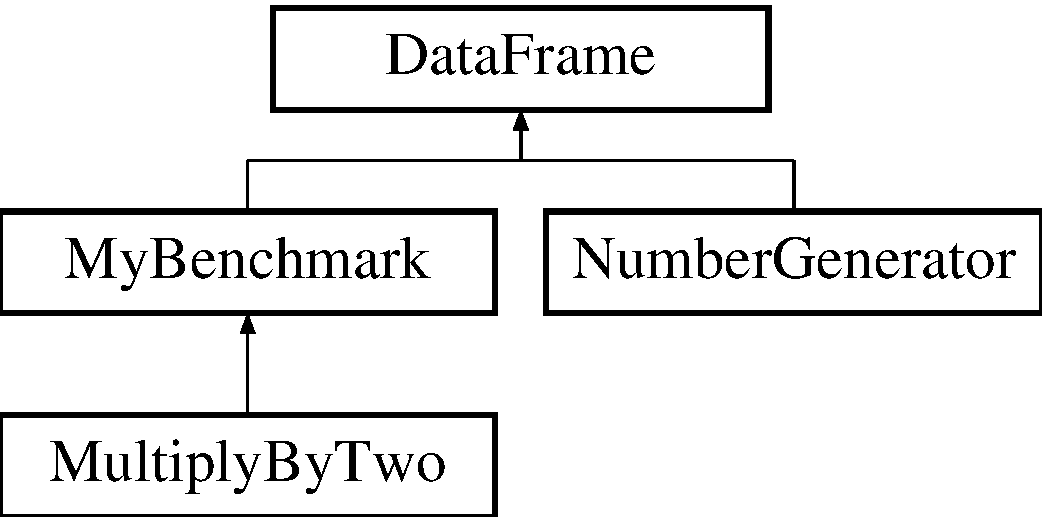
\includegraphics[height=3.000000cm]{class_data_frame}
\end{center}
\end{figure}
\subsubsection*{Metody publiczne}
\begin{DoxyCompactItemize}
\item 
\hyperlink{class_data_frame_a69a9dc47b7506b8062fd34aedacbf579}{Data\-Frame} ()
\begin{DoxyCompactList}\small\item\em Przypisuje zmiennym wartosci domyslne. \end{DoxyCompactList}\item 
int \hyperlink{class_data_frame_a617ef21804065f31115c01527155f499}{load\-Data\-From\-File} ()
\begin{DoxyCompactList}\small\item\em Ładuje dane z pliku. \end{DoxyCompactList}\item 
int \hyperlink{class_data_frame_a03cc3ac606fdb8a2dbcaea5d429cf208}{save\-Data\-To\-File} ()
\begin{DoxyCompactList}\small\item\em Zapisuje dane do pliku. \end{DoxyCompactList}\item 
\hyperlink{class_data_frame}{Data\-Frame} \hyperlink{class_data_frame_ab7dddb09f5ee9dc4a5783136dad01962}{operator=} (\hyperlink{class_data_frame}{Data\-Frame} dataframe)
\begin{DoxyCompactList}\small\item\em Kopiuje elementy roznych obiektow. \end{DoxyCompactList}\item 
virtual \hyperlink{class_data_frame_a1360ddf00d717392fe1292bc1e1990ff}{$\sim$\-Data\-Frame} ()
\end{DoxyCompactItemize}
\subsubsection*{Atrybuty publiczne}
\begin{DoxyCompactItemize}
\item 
int $\ast$ \hyperlink{class_data_frame_a8edc4ce524483e2e5069067267ccdcbf}{table\-Of\-Data}
\begin{DoxyCompactList}\small\item\em Zawiera adres do tablicy \{size\} elementów. \end{DoxyCompactList}\item 
char $\ast$ \hyperlink{class_data_frame_a824a73f019aec71281837abafd95a510}{output\-File\-Name}
\begin{DoxyCompactList}\small\item\em Zawiera nazwe pliku do zapisu. \end{DoxyCompactList}\item 
char $\ast$ \hyperlink{class_data_frame_a90041bfdf474b0d7ce39bc3dbbb55aa9}{input\-File\-Name}
\begin{DoxyCompactList}\small\item\em Zawiera nazwe pliku do odczytu. \end{DoxyCompactList}\item 
unsigned int \hyperlink{class_data_frame_aa5d1905c6910cad07ab5189bd34b13ab}{size\-Of\-Table}
\begin{DoxyCompactList}\small\item\em Rozmiar tablicy table\-Of\-Data. \end{DoxyCompactList}\end{DoxyCompactItemize}


\subsubsection{Opis szczegółowy}


Definicja w linii \hyperlink{dataframe_8h_source_l00015}{15} pliku \hyperlink{dataframe_8h_source}{dataframe.\-h}.



\subsubsection{Dokumentacja konstruktora i destruktora}
\hypertarget{class_data_frame_a69a9dc47b7506b8062fd34aedacbf579}{\index{Data\-Frame@{Data\-Frame}!Data\-Frame@{Data\-Frame}}
\index{Data\-Frame@{Data\-Frame}!DataFrame@{Data\-Frame}}
\paragraph[{Data\-Frame}]{\setlength{\rightskip}{0pt plus 5cm}Data\-Frame\-::\-Data\-Frame (
\begin{DoxyParamCaption}
{}
\end{DoxyParamCaption}
)}}\label{class_data_frame_a69a9dc47b7506b8062fd34aedacbf579}


Definicja w linii \hyperlink{dataframe_8cpp_source_l00012}{12} pliku \hyperlink{dataframe_8cpp_source}{dataframe.\-cpp}.



Odwołuje się do \hyperlink{dataframe_8h_source_l00029}{input\-File\-Name}, \hyperlink{dataframe_8h_source_l00025}{output\-File\-Name}, \hyperlink{dataframe_8h_source_l00034}{size\-Of\-Table} i \hyperlink{dataframe_8h_source_l00021}{table\-Of\-Data}.


\begin{DoxyCode}
00013 \{
00014         \hyperlink{class_data_frame_a8edc4ce524483e2e5069067267ccdcbf}{tableOfData} = 0;
00015         \hyperlink{class_data_frame_a824a73f019aec71281837abafd95a510}{outputFileName} = NULL;
00016         \hyperlink{class_data_frame_a90041bfdf474b0d7ce39bc3dbbb55aa9}{inputFileName} = NULL;
00017         \hyperlink{class_data_frame_aa5d1905c6910cad07ab5189bd34b13ab}{sizeOfTable} = 0;
00018 \}
\end{DoxyCode}
\hypertarget{class_data_frame_a1360ddf00d717392fe1292bc1e1990ff}{\index{Data\-Frame@{Data\-Frame}!$\sim$\-Data\-Frame@{$\sim$\-Data\-Frame}}
\index{$\sim$\-Data\-Frame@{$\sim$\-Data\-Frame}!DataFrame@{Data\-Frame}}
\paragraph[{$\sim$\-Data\-Frame}]{\setlength{\rightskip}{0pt plus 5cm}virtual Data\-Frame\-::$\sim$\-Data\-Frame (
\begin{DoxyParamCaption}
{}
\end{DoxyParamCaption}
)\hspace{0.3cm}{\ttfamily [inline]}, {\ttfamily [virtual]}}}\label{class_data_frame_a1360ddf00d717392fe1292bc1e1990ff}


Definicja w linii \hyperlink{dataframe_8h_source_l00064}{64} pliku \hyperlink{dataframe_8h_source}{dataframe.\-h}.


\begin{DoxyCode}
00064 \{\}
\end{DoxyCode}


\subsubsection{Dokumentacja funkcji składowych}
\hypertarget{class_data_frame_a617ef21804065f31115c01527155f499}{\index{Data\-Frame@{Data\-Frame}!load\-Data\-From\-File@{load\-Data\-From\-File}}
\index{load\-Data\-From\-File@{load\-Data\-From\-File}!DataFrame@{Data\-Frame}}
\paragraph[{load\-Data\-From\-File}]{\setlength{\rightskip}{0pt plus 5cm}int Data\-Frame\-::load\-Data\-From\-File (
\begin{DoxyParamCaption}
{}
\end{DoxyParamCaption}
)}}\label{class_data_frame_a617ef21804065f31115c01527155f499}
Wczytuje dane z pliku i zapisuje je dynamicznie do tablicy jednowymiarowej, na ktora wskazuje wskaźnik $\ast$table\-Of\-Data

Rozmiar tablicy jest przechowywany w size\-Of\-Table 

Definicja w linii \hyperlink{dataframe_8cpp_source_l00020}{20} pliku \hyperlink{dataframe_8cpp_source}{dataframe.\-cpp}.



Odwołuje się do \hyperlink{dataframe_8h_source_l00029}{input\-File\-Name}, \hyperlink{dataframe_8h_source_l00034}{size\-Of\-Table} i \hyperlink{dataframe_8h_source_l00021}{table\-Of\-Data}.


\begin{DoxyCode}
00021 \{
00022         std::ifstream streamToFile;
00023         streamToFile.open (\hyperlink{class_data_frame_a90041bfdf474b0d7ce39bc3dbbb55aa9}{inputFileName}, std::ifstream::in);
00024         this->\hyperlink{class_data_frame_a8edc4ce524483e2e5069067267ccdcbf}{tableOfData} = \textcolor{keyword}{new} \textcolor{keywordtype}{int}[\hyperlink{class_data_frame_aa5d1905c6910cad07ab5189bd34b13ab}{sizeOfTable}];
00025         \textcolor{keywordflow}{for}(\textcolor{keywordtype}{unsigned} \textcolor{keywordtype}{int} i=0; i<\hyperlink{class_data_frame_aa5d1905c6910cad07ab5189bd34b13ab}{sizeOfTable} ; i++) \{
00026                 streamToFile >> this-> \hyperlink{class_data_frame_a8edc4ce524483e2e5069067267ccdcbf}{tableOfData}[i];
00027                 \textcolor{keywordflow}{if} (streamToFile.eof()) \textcolor{keywordflow}{return} 1; \textcolor{comment}{//[EoF reached]}
00028         \}
00029         \textcolor{keywordflow}{return} 0;
00030 \}
\end{DoxyCode}
\hypertarget{class_data_frame_ab7dddb09f5ee9dc4a5783136dad01962}{\index{Data\-Frame@{Data\-Frame}!operator=@{operator=}}
\index{operator=@{operator=}!DataFrame@{Data\-Frame}}
\paragraph[{operator=}]{\setlength{\rightskip}{0pt plus 5cm}{\bf Data\-Frame} Data\-Frame\-::operator= (
\begin{DoxyParamCaption}
\item[{{\bf Data\-Frame}}]{dataframe}
\end{DoxyParamCaption}
)}}\label{class_data_frame_ab7dddb09f5ee9dc4a5783136dad01962}
Zapisuje kolejne liczby do pliku o nazwie output\-File\-Name 

Definicja w linii \hyperlink{dataframe_8cpp_source_l00044}{44} pliku \hyperlink{dataframe_8cpp_source}{dataframe.\-cpp}.



Odwołuje się do \hyperlink{dataframe_8h_source_l00029}{input\-File\-Name}, \hyperlink{dataframe_8h_source_l00025}{output\-File\-Name}, \hyperlink{dataframe_8h_source_l00034}{size\-Of\-Table} i \hyperlink{dataframe_8h_source_l00021}{table\-Of\-Data}.


\begin{DoxyCode}
00045 \{
00046         this->\hyperlink{class_data_frame_a8edc4ce524483e2e5069067267ccdcbf}{tableOfData} = dataframe.\hyperlink{class_data_frame_a8edc4ce524483e2e5069067267ccdcbf}{tableOfData};
00047         this->\hyperlink{class_data_frame_a824a73f019aec71281837abafd95a510}{outputFileName} = dataframe.\hyperlink{class_data_frame_a824a73f019aec71281837abafd95a510}{outputFileName};
00048         this->\hyperlink{class_data_frame_a90041bfdf474b0d7ce39bc3dbbb55aa9}{inputFileName} = dataframe.\hyperlink{class_data_frame_a90041bfdf474b0d7ce39bc3dbbb55aa9}{inputFileName};
00049         this->\hyperlink{class_data_frame_aa5d1905c6910cad07ab5189bd34b13ab}{sizeOfTable} = dataframe.\hyperlink{class_data_frame_aa5d1905c6910cad07ab5189bd34b13ab}{sizeOfTable};
00050         \textcolor{keywordflow}{return} *\textcolor{keyword}{this};
00051 \}
\end{DoxyCode}
\hypertarget{class_data_frame_a03cc3ac606fdb8a2dbcaea5d429cf208}{\index{Data\-Frame@{Data\-Frame}!save\-Data\-To\-File@{save\-Data\-To\-File}}
\index{save\-Data\-To\-File@{save\-Data\-To\-File}!DataFrame@{Data\-Frame}}
\paragraph[{save\-Data\-To\-File}]{\setlength{\rightskip}{0pt plus 5cm}int Data\-Frame\-::save\-Data\-To\-File (
\begin{DoxyParamCaption}
{}
\end{DoxyParamCaption}
)}}\label{class_data_frame_a03cc3ac606fdb8a2dbcaea5d429cf208}
Wczytuje liczby z pliku o nazwie intput\-File\-Name 

Definicja w linii \hyperlink{dataframe_8cpp_source_l00032}{32} pliku \hyperlink{dataframe_8cpp_source}{dataframe.\-cpp}.



Odwołuje się do \hyperlink{dataframe_8h_source_l00025}{output\-File\-Name}, \hyperlink{dataframe_8h_source_l00034}{size\-Of\-Table} i \hyperlink{dataframe_8h_source_l00021}{table\-Of\-Data}.


\begin{DoxyCode}
00033 \{
00034         std::ofstream streamToFile;
00035         streamToFile.open (\hyperlink{class_data_frame_a824a73f019aec71281837abafd95a510}{outputFileName}, std::ofstream::out);
00036         \textcolor{keywordflow}{for}(\textcolor{keywordtype}{unsigned} \textcolor{keywordtype}{int} i=0; i<\hyperlink{class_data_frame_aa5d1905c6910cad07ab5189bd34b13ab}{sizeOfTable} ; i++) \{
00037                 streamToFile << this-> \hyperlink{class_data_frame_a8edc4ce524483e2e5069067267ccdcbf}{tableOfData}[i] <<\textcolor{charliteral}{' '};
00038         \}
00039         \textcolor{keywordflow}{return} 0;
00040 \}
\end{DoxyCode}


\subsubsection{Dokumentacja atrybutów składowych}
\hypertarget{class_data_frame_a90041bfdf474b0d7ce39bc3dbbb55aa9}{\index{Data\-Frame@{Data\-Frame}!input\-File\-Name@{input\-File\-Name}}
\index{input\-File\-Name@{input\-File\-Name}!DataFrame@{Data\-Frame}}
\paragraph[{input\-File\-Name}]{\setlength{\rightskip}{0pt plus 5cm}char$\ast$ Data\-Frame\-::input\-File\-Name}}\label{class_data_frame_a90041bfdf474b0d7ce39bc3dbbb55aa9}


Definicja w linii \hyperlink{dataframe_8h_source_l00029}{29} pliku \hyperlink{dataframe_8h_source}{dataframe.\-h}.



Odwołania w \hyperlink{dataframe_8cpp_source_l00012}{Data\-Frame()}, \hyperlink{dataframe_8cpp_source_l00020}{load\-Data\-From\-File()}, \hyperlink{main_8cpp_source_l00019}{main()} i \hyperlink{dataframe_8cpp_source_l00044}{operator=()}.

\hypertarget{class_data_frame_a824a73f019aec71281837abafd95a510}{\index{Data\-Frame@{Data\-Frame}!output\-File\-Name@{output\-File\-Name}}
\index{output\-File\-Name@{output\-File\-Name}!DataFrame@{Data\-Frame}}
\paragraph[{output\-File\-Name}]{\setlength{\rightskip}{0pt plus 5cm}char$\ast$ Data\-Frame\-::output\-File\-Name}}\label{class_data_frame_a824a73f019aec71281837abafd95a510}


Definicja w linii \hyperlink{dataframe_8h_source_l00025}{25} pliku \hyperlink{dataframe_8h_source}{dataframe.\-h}.



Odwołania w \hyperlink{dataframe_8cpp_source_l00012}{Data\-Frame()}, \hyperlink{main_8cpp_source_l00019}{main()}, \hyperlink{dataframe_8cpp_source_l00044}{operator=()} i \hyperlink{dataframe_8cpp_source_l00032}{save\-Data\-To\-File()}.

\hypertarget{class_data_frame_aa5d1905c6910cad07ab5189bd34b13ab}{\index{Data\-Frame@{Data\-Frame}!size\-Of\-Table@{size\-Of\-Table}}
\index{size\-Of\-Table@{size\-Of\-Table}!DataFrame@{Data\-Frame}}
\paragraph[{size\-Of\-Table}]{\setlength{\rightskip}{0pt plus 5cm}unsigned int Data\-Frame\-::size\-Of\-Table}}\label{class_data_frame_aa5d1905c6910cad07ab5189bd34b13ab}


Definicja w linii \hyperlink{dataframe_8h_source_l00034}{34} pliku \hyperlink{dataframe_8h_source}{dataframe.\-h}.



Odwołania w \hyperlink{dataframe_8cpp_source_l00012}{Data\-Frame()}, \hyperlink{multiplybytwo_8cpp_source_l00011}{Multiply\-By\-Two\-::execute\-Algorithm()}, \hyperlink{numbergenerator_8h_source_l00031}{Number\-Generator\-::generate\-Numbers()}, \hyperlink{dataframe_8cpp_source_l00020}{load\-Data\-From\-File()}, \hyperlink{main_8cpp_source_l00019}{main()}, \hyperlink{dataframe_8cpp_source_l00044}{operator=()}, \hyperlink{dataframe_8cpp_source_l00032}{save\-Data\-To\-File()} i \hyperlink{mybenchmark_8cpp_source_l00012}{My\-Benchmark\-::test\-Algorithm()}.

\hypertarget{class_data_frame_a8edc4ce524483e2e5069067267ccdcbf}{\index{Data\-Frame@{Data\-Frame}!table\-Of\-Data@{table\-Of\-Data}}
\index{table\-Of\-Data@{table\-Of\-Data}!DataFrame@{Data\-Frame}}
\paragraph[{table\-Of\-Data}]{\setlength{\rightskip}{0pt plus 5cm}int$\ast$ Data\-Frame\-::table\-Of\-Data}}\label{class_data_frame_a8edc4ce524483e2e5069067267ccdcbf}


Definicja w linii \hyperlink{dataframe_8h_source_l00021}{21} pliku \hyperlink{dataframe_8h_source}{dataframe.\-h}.



Odwołania w \hyperlink{dataframe_8cpp_source_l00012}{Data\-Frame()}, \hyperlink{multiplybytwo_8cpp_source_l00011}{Multiply\-By\-Two\-::execute\-Algorithm()}, \hyperlink{numbergenerator_8h_source_l00031}{Number\-Generator\-::generate\-Numbers()}, \hyperlink{dataframe_8cpp_source_l00020}{load\-Data\-From\-File()}, \hyperlink{dataframe_8cpp_source_l00044}{operator=()}, \hyperlink{dataframe_8cpp_source_l00032}{save\-Data\-To\-File()} i \hyperlink{mybenchmark_8cpp_source_l00012}{My\-Benchmark\-::test\-Algorithm()}.



Dokumentacja dla tej klasy została wygenerowana z plików\-:\begin{DoxyCompactItemize}
\item 
\hyperlink{dataframe_8h}{dataframe.\-h}\item 
\hyperlink{dataframe_8cpp}{dataframe.\-cpp}\end{DoxyCompactItemize}

\hypertarget{class_multiply_by_two}{\subsection{Dokumentacja klasy Multiply\-By\-Two}
\label{class_multiply_by_two}\index{Multiply\-By\-Two@{Multiply\-By\-Two}}
}


Algorytm mnozy kazda liczbe razy 2.  




{\ttfamily \#include $<$multiplybytwo.\-h$>$}

Diagram dziedziczenia dla Multiply\-By\-Two\begin{figure}[H]
\begin{center}
\leavevmode
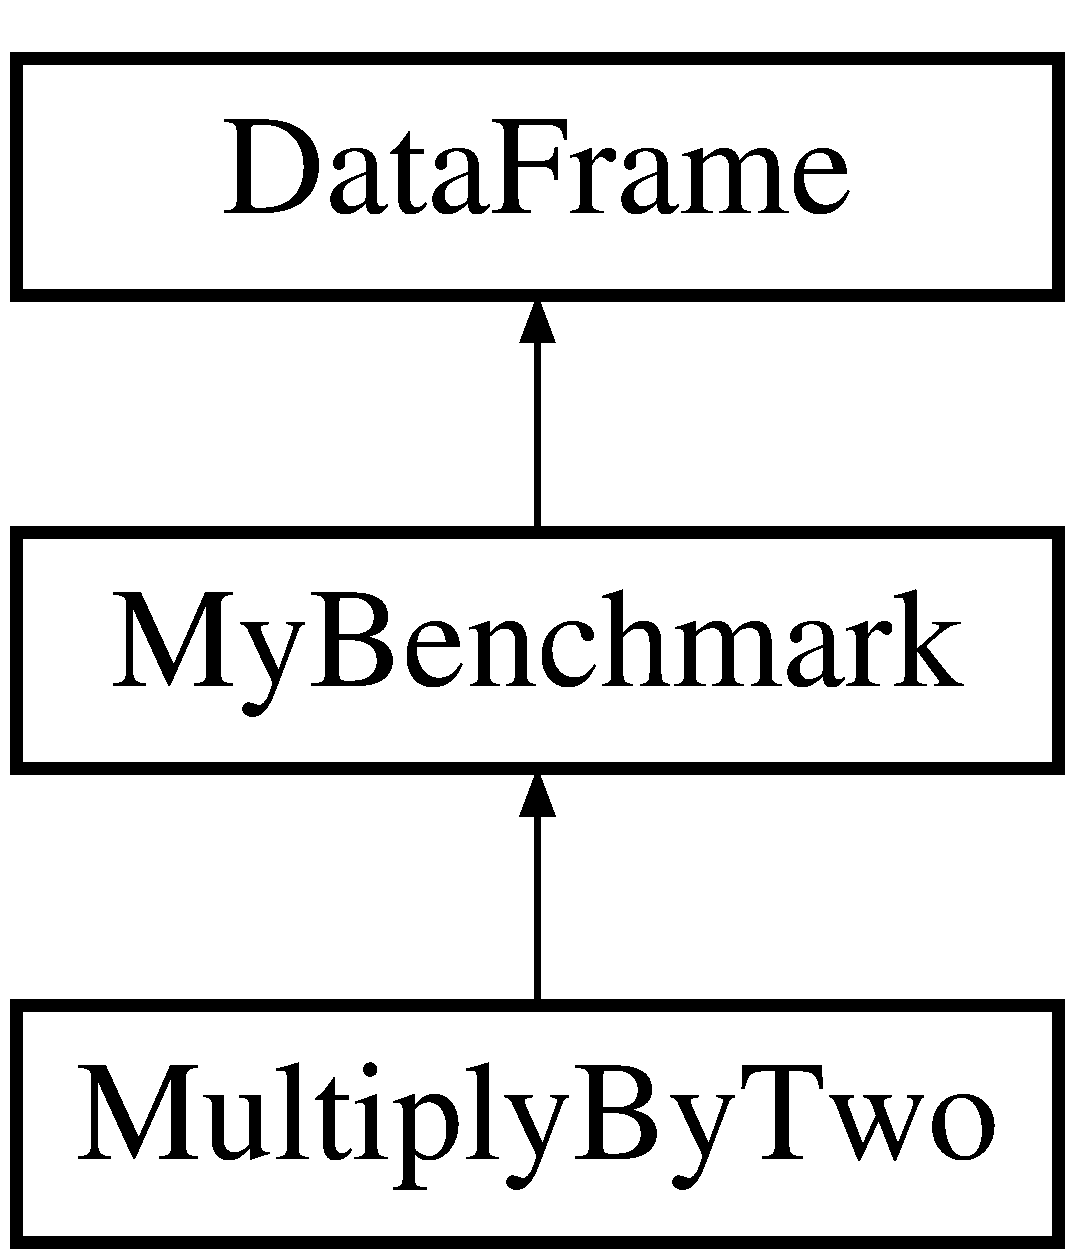
\includegraphics[height=3.000000cm]{class_multiply_by_two}
\end{center}
\end{figure}
\subsubsection*{Metody publiczne}
\begin{DoxyCompactItemize}
\item 
void \hyperlink{class_multiply_by_two_aad2080a1fdab088814170e529a14db1e}{execute\-Algorithm} ()
\begin{DoxyCompactList}\small\item\em Wykonuje algorytm mnozenie x2. \end{DoxyCompactList}\item 
\hyperlink{class_multiply_by_two_ab84d2c946e0ac7d6eeef32d5800ce4a5}{$\sim$\-Multiply\-By\-Two} ()
\end{DoxyCompactItemize}
\subsubsection*{Dodatkowe Dziedziczone Składowe}


\subsubsection{Opis szczegółowy}
Algorytm mnozy kazda kolejna liczbe przez 2 

Definicja w linii \hyperlink{multiplybytwo_8h_source_l00020}{20} pliku \hyperlink{multiplybytwo_8h_source}{multiplybytwo.\-h}.



\subsubsection{Dokumentacja konstruktora i destruktora}
\hypertarget{class_multiply_by_two_ab84d2c946e0ac7d6eeef32d5800ce4a5}{\index{Multiply\-By\-Two@{Multiply\-By\-Two}!$\sim$\-Multiply\-By\-Two@{$\sim$\-Multiply\-By\-Two}}
\index{$\sim$\-Multiply\-By\-Two@{$\sim$\-Multiply\-By\-Two}!MultiplyByTwo@{Multiply\-By\-Two}}
\paragraph[{$\sim$\-Multiply\-By\-Two}]{\setlength{\rightskip}{0pt plus 5cm}Multiply\-By\-Two\-::$\sim$\-Multiply\-By\-Two (
\begin{DoxyParamCaption}
{}
\end{DoxyParamCaption}
)\hspace{0.3cm}{\ttfamily [inline]}}}\label{class_multiply_by_two_ab84d2c946e0ac7d6eeef32d5800ce4a5}


Definicja w linii \hyperlink{multiplybytwo_8h_source_l00029}{29} pliku \hyperlink{multiplybytwo_8h_source}{multiplybytwo.\-h}.


\begin{DoxyCode}
00029 \{\}
\end{DoxyCode}


\subsubsection{Dokumentacja funkcji składowych}
\hypertarget{class_multiply_by_two_aad2080a1fdab088814170e529a14db1e}{\index{Multiply\-By\-Two@{Multiply\-By\-Two}!execute\-Algorithm@{execute\-Algorithm}}
\index{execute\-Algorithm@{execute\-Algorithm}!MultiplyByTwo@{Multiply\-By\-Two}}
\paragraph[{execute\-Algorithm}]{\setlength{\rightskip}{0pt plus 5cm}void Multiply\-By\-Two\-::execute\-Algorithm (
\begin{DoxyParamCaption}
{}
\end{DoxyParamCaption}
)\hspace{0.3cm}{\ttfamily [virtual]}}}\label{class_multiply_by_two_aad2080a1fdab088814170e529a14db1e}


Implementuje \hyperlink{class_my_benchmark_aaebbb9785ed7c460e33459464655a611}{My\-Benchmark}.



Definicja w linii \hyperlink{multiplybytwo_8cpp_source_l00011}{11} pliku \hyperlink{multiplybytwo_8cpp_source}{multiplybytwo.\-cpp}.



Odwołuje się do \hyperlink{dataframe_8h_source_l00034}{Data\-Frame\-::size\-Of\-Table} i \hyperlink{dataframe_8h_source_l00021}{Data\-Frame\-::table\-Of\-Data}.


\begin{DoxyCode}
00012 \{
00013         \textcolor{keywordflow}{for}(\textcolor{keywordtype}{unsigned} \textcolor{keywordtype}{int} i=0; i<\hyperlink{class_data_frame_aa5d1905c6910cad07ab5189bd34b13ab}{sizeOfTable}; i++) \{
00014 
00015                 \hyperlink{class_data_frame_a8edc4ce524483e2e5069067267ccdcbf}{tableOfData}[i]*=2;
00016         \}
00017 
00018 
00019 
00020 \}
\end{DoxyCode}


Dokumentacja dla tej klasy została wygenerowana z plików\-:\begin{DoxyCompactItemize}
\item 
\hyperlink{multiplybytwo_8h}{multiplybytwo.\-h}\item 
\hyperlink{multiplybytwo_8cpp}{multiplybytwo.\-cpp}\end{DoxyCompactItemize}

\hypertarget{class_my_benchmark}{\section{Dokumentacja klasy My\-Benchmark}
\label{class_my_benchmark}\index{My\-Benchmark@{My\-Benchmark}}
}


Klasa bazowa/interface do testowania algorytmu.  




{\ttfamily \#include $<$mybenchmark.\-h$>$}

Diagram dziedziczenia dla My\-Benchmark\begin{figure}[H]
\begin{center}
\leavevmode
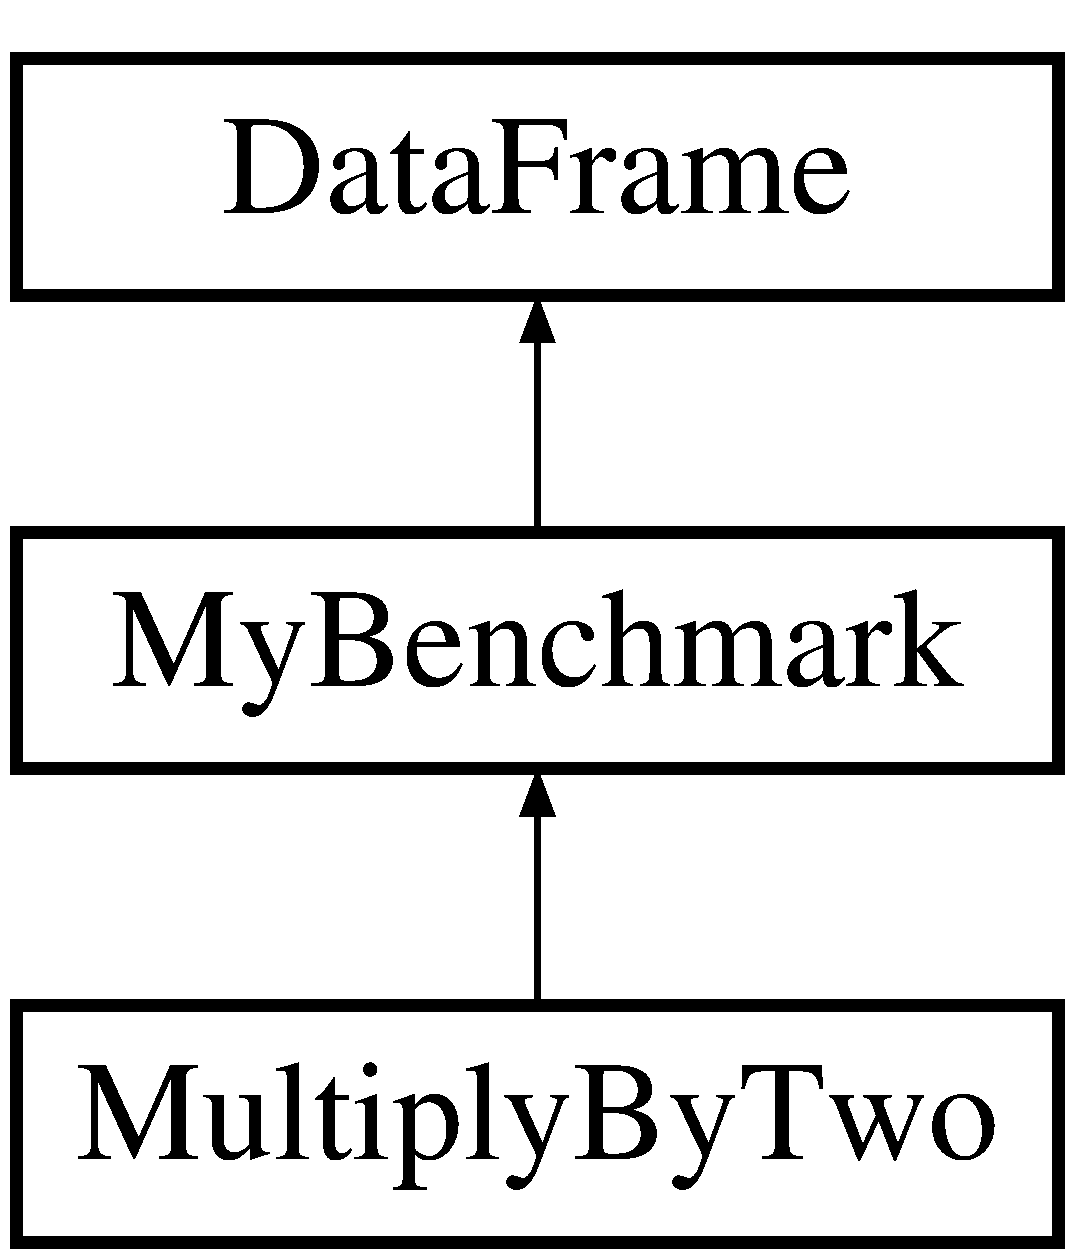
\includegraphics[height=3.000000cm]{class_my_benchmark}
\end{center}
\end{figure}
\subsection*{Metody publiczne}
\begin{DoxyCompactItemize}
\item 
double \hyperlink{class_my_benchmark_a66576625ca37f8bc539c18ffceb69c9c}{test\-Algorithm} (unsigned int repetition)
\begin{DoxyCompactList}\small\item\em Benchmarkuje algorytm główny. \end{DoxyCompactList}\item 
virtual \hyperlink{class_my_benchmark_a00de82c40680b41065eb402ac90f1736}{$\sim$\-My\-Benchmark} ()
\begin{DoxyCompactList}\small\item\em Usuwam obiekt test biorąc pod uwage jego prawdziwy typ. \end{DoxyCompactList}\end{DoxyCompactItemize}
\subsection*{Metody chronione}
\begin{DoxyCompactItemize}
\item 
virtual void \hyperlink{class_my_benchmark_aaebbb9785ed7c460e33459464655a611}{execute\-Algorithm} ()=0
\begin{DoxyCompactList}\small\item\em Interface metody algorytmu glownego. \end{DoxyCompactList}\end{DoxyCompactItemize}
\subsection*{Dodatkowe Dziedziczone Składowe}


\subsection{Opis szczegółowy}
Używana jako interface dla wszystkich algorytmow aby testowac czas wykonywanego algorymtu. 

Definicja w linii 20 pliku mybenchmark.\-h.



\subsection{Dokumentacja konstruktora i destruktora}
\hypertarget{class_my_benchmark_a00de82c40680b41065eb402ac90f1736}{\index{My\-Benchmark@{My\-Benchmark}!$\sim$\-My\-Benchmark@{$\sim$\-My\-Benchmark}}
\index{$\sim$\-My\-Benchmark@{$\sim$\-My\-Benchmark}!MyBenchmark@{My\-Benchmark}}
\subsubsection[{$\sim$\-My\-Benchmark}]{\setlength{\rightskip}{0pt plus 5cm}virtual My\-Benchmark\-::$\sim$\-My\-Benchmark (
\begin{DoxyParamCaption}
{}
\end{DoxyParamCaption}
)\hspace{0.3cm}{\ttfamily [inline]}, {\ttfamily [virtual]}}}\label{class_my_benchmark_a00de82c40680b41065eb402ac90f1736}


Definicja w linii 49 pliku mybenchmark.\-h.



\subsection{Dokumentacja funkcji składowych}
\hypertarget{class_my_benchmark_aaebbb9785ed7c460e33459464655a611}{\index{My\-Benchmark@{My\-Benchmark}!execute\-Algorithm@{execute\-Algorithm}}
\index{execute\-Algorithm@{execute\-Algorithm}!MyBenchmark@{My\-Benchmark}}
\subsubsection[{execute\-Algorithm}]{\setlength{\rightskip}{0pt plus 5cm}virtual void My\-Benchmark\-::execute\-Algorithm (
\begin{DoxyParamCaption}
{}
\end{DoxyParamCaption}
)\hspace{0.3cm}{\ttfamily [protected]}, {\ttfamily [pure virtual]}}}\label{class_my_benchmark_aaebbb9785ed7c460e33459464655a611}
Metoda abstrakcyjna, ktora jest interfacem do implementacji przez glowny algorytm. To znaczy, ze kazdy algorytm ma byc uruchamiany tą funkcja 

Implementowany w \hyperlink{class_multiply_by_two_aad2080a1fdab088814170e529a14db1e}{Multiply\-By\-Two}.

\hypertarget{class_my_benchmark_a66576625ca37f8bc539c18ffceb69c9c}{\index{My\-Benchmark@{My\-Benchmark}!test\-Algorithm@{test\-Algorithm}}
\index{test\-Algorithm@{test\-Algorithm}!MyBenchmark@{My\-Benchmark}}
\subsubsection[{test\-Algorithm}]{\setlength{\rightskip}{0pt plus 5cm}double My\-Benchmark\-::test\-Algorithm (
\begin{DoxyParamCaption}
\item[{unsigned int}]{repetition}
\end{DoxyParamCaption}
)}}\label{class_my_benchmark_a66576625ca37f8bc539c18ffceb69c9c}
Obliczam czas wykonywanego algorytmu dzięki zastosowaniu metody abstrakcyjnej \hyperlink{class_my_benchmark_aaebbb9785ed7c460e33459464655a611}{execute\-Algorithm()} i zaimplementowaniu tego interfacu w algorytmie głównym 

Definicja w linii 12 pliku mybenchmark.\-cpp.



Dokumentacja dla tej klasy została wygenerowana z plików\-:\begin{DoxyCompactItemize}
\item 
\hyperlink{mybenchmark_8h}{mybenchmark.\-h}\item 
\hyperlink{mybenchmark_8cpp}{mybenchmark.\-cpp}\end{DoxyCompactItemize}

\hypertarget{class_my_list}{\subsection{Dokumentacja klasy My\-List}
\label{class_my_list}\index{My\-List@{My\-List}}
}


Lista dwukierunkowa.  




{\ttfamily \#include $<$mylist.\-h$>$}

Diagram dziedziczenia dla My\-List\begin{figure}[H]
\begin{center}
\leavevmode
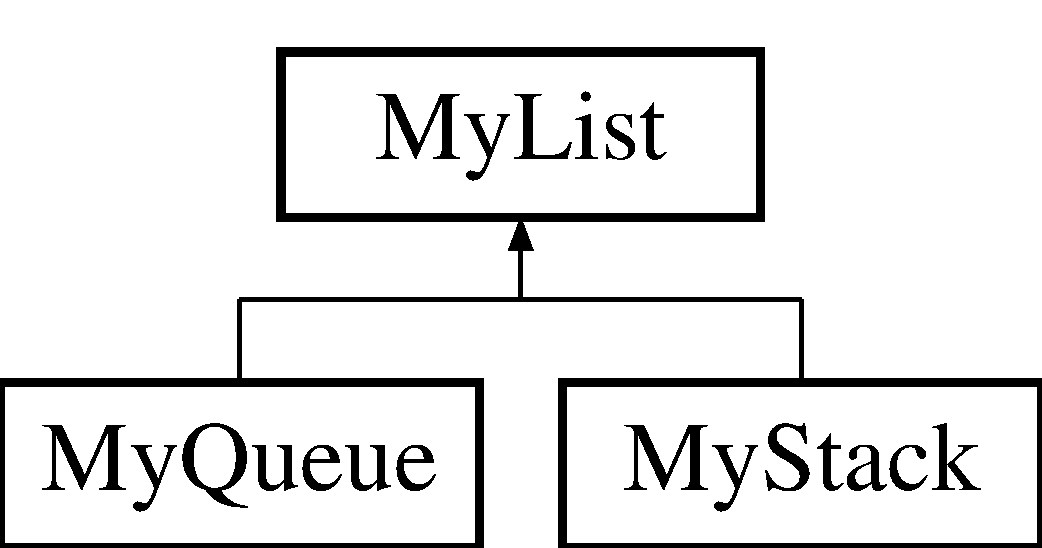
\includegraphics[height=2.000000cm]{class_my_list}
\end{center}
\end{figure}
\subsubsection*{Komponenty}
\begin{DoxyCompactItemize}
\item 
class \hyperlink{class_my_list_1_1_my_list_element}{My\-List\-Element}
\begin{DoxyCompactList}\small\item\em Klasa 'malych struktur' gdzie jest numer i wskaznik do nas elementu. \end{DoxyCompactList}\end{DoxyCompactItemize}
\subsubsection*{Metody publiczne}
\begin{DoxyCompactItemize}
\item 
\hyperlink{class_my_list_ae9cd2a6b068e02fa39ba3e539425c1c1}{My\-List} ()
\begin{DoxyCompactList}\small\item\em Konstruktor listy. \end{DoxyCompactList}\item 
int \hyperlink{class_my_list_a6d21c8bfbd9cd31efdba81ba488f43f2}{size} ()
\begin{DoxyCompactList}\small\item\em Zwraca ilosc elementow listy. \end{DoxyCompactList}\item 
int \hyperlink{class_my_list_a7361ad3b0da0402cb95adb225ebfaffd}{pop\-\_\-back} ()
\begin{DoxyCompactList}\small\item\em Zwraca element ostatni w liscie. \end{DoxyCompactList}\item 
int \hyperlink{class_my_list_ae038b14e6cb5b54b8499b85ce5f03a0e}{pop\-\_\-front} ()
\begin{DoxyCompactList}\small\item\em Zwraca element pierwszy w liscie. \end{DoxyCompactList}\item 
void \hyperlink{class_my_list_a8428cca9d08fcf02e378aee0a232e971}{push\-\_\-back} (int arg)
\begin{DoxyCompactList}\small\item\em Wklada element na ostatnie miejsce na liscie. \end{DoxyCompactList}\item 
void \hyperlink{class_my_list_a9ab5ae823e85df90662e42fab4229f09}{push\-\_\-front} (int arg)
\begin{DoxyCompactList}\small\item\em Wklada element na pierwsze miejsce na liscie. \end{DoxyCompactList}\end{DoxyCompactItemize}
\subsubsection*{Atrybuty prywatne}
\begin{DoxyCompactItemize}
\item 
int \hyperlink{class_my_list_a77b7870f617b51fad7399463c9147668}{size\-Of\-List}
\begin{DoxyCompactList}\small\item\em liczba elementow listy \end{DoxyCompactList}\item 
\hyperlink{class_my_list_1_1_my_list_element}{My\-List\-Element} $\ast$ \hyperlink{class_my_list_aa7e5ddd2dddeeccd304126130d73dead}{first\-Element}
\begin{DoxyCompactList}\small\item\em wskaznik do 'malej struktury' ktora jest pierwsza na liscie \end{DoxyCompactList}\item 
\hyperlink{class_my_list_1_1_my_list_element}{My\-List\-Element} $\ast$ \hyperlink{class_my_list_a287894c4add6b52be99826fb4d76594c}{last\-Element}
\begin{DoxyCompactList}\small\item\em wskaznik do 'malej struktury' ktora jest ostatnia na liscie \end{DoxyCompactList}\end{DoxyCompactItemize}


\subsubsection{Opis szczegółowy}
Klasa przedstawia liste dwukierunkową dynamiczna 

Definicja w linii \hyperlink{mylist_8h_source_l00018}{18} pliku \hyperlink{mylist_8h_source}{mylist.\-h}.



\subsubsection{Dokumentacja konstruktora i destruktora}
\hypertarget{class_my_list_ae9cd2a6b068e02fa39ba3e539425c1c1}{\index{My\-List@{My\-List}!My\-List@{My\-List}}
\index{My\-List@{My\-List}!MyList@{My\-List}}
\paragraph[{My\-List}]{\setlength{\rightskip}{0pt plus 5cm}My\-List\-::\-My\-List (
\begin{DoxyParamCaption}
{}
\end{DoxyParamCaption}
)}}\label{class_my_list_ae9cd2a6b068e02fa39ba3e539425c1c1}


Definicja w linii \hyperlink{mylist_8cpp_source_l00011}{11} pliku \hyperlink{mylist_8cpp_source}{mylist.\-cpp}.



Odwołuje się do \hyperlink{mylist_8h_source_l00043}{first\-Element}, \hyperlink{mylist_8h_source_l00045}{last\-Element} i \hyperlink{mylist_8h_source_l00022}{size\-Of\-List}.


\begin{DoxyCode}
00012 \{
00013         \hyperlink{class_my_list_aa7e5ddd2dddeeccd304126130d73dead}{firstElement} = \hyperlink{class_my_list_a287894c4add6b52be99826fb4d76594c}{lastElement} = \textcolor{keyword}{new} MyListElement(0);
00014         \hyperlink{class_my_list_a77b7870f617b51fad7399463c9147668}{sizeOfList} = 0;
00015 \}
\end{DoxyCode}


\subsubsection{Dokumentacja funkcji składowych}
\hypertarget{class_my_list_a7361ad3b0da0402cb95adb225ebfaffd}{\index{My\-List@{My\-List}!pop\-\_\-back@{pop\-\_\-back}}
\index{pop\-\_\-back@{pop\-\_\-back}!MyList@{My\-List}}
\paragraph[{pop\-\_\-back}]{\setlength{\rightskip}{0pt plus 5cm}int My\-List\-::pop\-\_\-back (
\begin{DoxyParamCaption}
{}
\end{DoxyParamCaption}
)}}\label{class_my_list_a7361ad3b0da0402cb95adb225ebfaffd}
\begin{DoxyReturn}{Zwraca}
Zwraca element ostatni w liscie 
\end{DoxyReturn}


Definicja w linii \hyperlink{mylist_8cpp_source_l00037}{37} pliku \hyperlink{mylist_8cpp_source}{mylist.\-cpp}.



Odwołuje się do \hyperlink{mylist_8h_source_l00045}{last\-Element} i \hyperlink{mylist_8h_source_l00022}{size\-Of\-List}.



Odwołania w \hyperlink{mystack_8h_source_l00029}{My\-Stack\-::pop()}.


\begin{DoxyCode}
00038 \{
00039         \textcolor{keywordflow}{if}(!(\hyperlink{class_my_list_a77b7870f617b51fad7399463c9147668}{sizeOfList}--)) \{ \hyperlink{class_my_list_a77b7870f617b51fad7399463c9147668}{sizeOfList}=0; \textcolor{keywordflow}{return} 0; \}
00040         \textcolor{keywordtype}{int} tmpNumber = \textcolor{keyword}{this} -> \hyperlink{class_my_list_a287894c4add6b52be99826fb4d76594c}{lastElement} -> number;
00041         MyListElement *originMyListElement = \textcolor{keyword}{this} -> \hyperlink{class_my_list_a287894c4add6b52be99826fb4d76594c}{lastElement};
00042         \textcolor{keyword}{this} -> \hyperlink{class_my_list_a287894c4add6b52be99826fb4d76594c}{lastElement} = \textcolor{keyword}{this} -> \hyperlink{class_my_list_a287894c4add6b52be99826fb4d76594c}{lastElement} -> previousElement;
00043         \textcolor{keyword}{delete} originMyListElement;
00044         \textcolor{keywordflow}{return} tmpNumber;
00045 \}
\end{DoxyCode}
\hypertarget{class_my_list_ae038b14e6cb5b54b8499b85ce5f03a0e}{\index{My\-List@{My\-List}!pop\-\_\-front@{pop\-\_\-front}}
\index{pop\-\_\-front@{pop\-\_\-front}!MyList@{My\-List}}
\paragraph[{pop\-\_\-front}]{\setlength{\rightskip}{0pt plus 5cm}int My\-List\-::pop\-\_\-front (
\begin{DoxyParamCaption}
{}
\end{DoxyParamCaption}
)}}\label{class_my_list_ae038b14e6cb5b54b8499b85ce5f03a0e}
\begin{DoxyReturn}{Zwraca}
Zwraca element pierwszy w liscie 
\end{DoxyReturn}


Definicja w linii \hyperlink{mylist_8cpp_source_l00046}{46} pliku \hyperlink{mylist_8cpp_source}{mylist.\-cpp}.



Odwołuje się do \hyperlink{mylist_8h_source_l00043}{first\-Element} i \hyperlink{mylist_8h_source_l00022}{size\-Of\-List}.



Odwołania w \hyperlink{myqueue_8h_source_l00027}{My\-Queue\-::pop()}.


\begin{DoxyCode}
00047 \{
00048         \textcolor{keywordflow}{if}(!(\hyperlink{class_my_list_a77b7870f617b51fad7399463c9147668}{sizeOfList}--)) \{ \hyperlink{class_my_list_a77b7870f617b51fad7399463c9147668}{sizeOfList}=0; \textcolor{keywordflow}{return} 0; \}
00049         \textcolor{keywordtype}{int} tmpNumber = \textcolor{keyword}{this} -> \hyperlink{class_my_list_aa7e5ddd2dddeeccd304126130d73dead}{firstElement} -> number;
00050         MyListElement *originMyListElement = \textcolor{keyword}{this} -> \hyperlink{class_my_list_aa7e5ddd2dddeeccd304126130d73dead}{firstElement};
00051         \textcolor{keyword}{this} -> \hyperlink{class_my_list_aa7e5ddd2dddeeccd304126130d73dead}{firstElement} = \textcolor{keyword}{this} -> \hyperlink{class_my_list_aa7e5ddd2dddeeccd304126130d73dead}{firstElement} -> nextElement;
00052 
00053         \textcolor{keyword}{delete} originMyListElement;
00054         \textcolor{keywordflow}{return} tmpNumber;
00055 \}
\end{DoxyCode}
\hypertarget{class_my_list_a8428cca9d08fcf02e378aee0a232e971}{\index{My\-List@{My\-List}!push\-\_\-back@{push\-\_\-back}}
\index{push\-\_\-back@{push\-\_\-back}!MyList@{My\-List}}
\paragraph[{push\-\_\-back}]{\setlength{\rightskip}{0pt plus 5cm}void My\-List\-::push\-\_\-back (
\begin{DoxyParamCaption}
\item[{int}]{arg}
\end{DoxyParamCaption}
)}}\label{class_my_list_a8428cca9d08fcf02e378aee0a232e971}


Definicja w linii \hyperlink{mylist_8cpp_source_l00018}{18} pliku \hyperlink{mylist_8cpp_source}{mylist.\-cpp}.



Odwołuje się do \hyperlink{mylist_8h_source_l00043}{first\-Element}, \hyperlink{mylist_8h_source_l00045}{last\-Element} i \hyperlink{mylist_8h_source_l00022}{size\-Of\-List}.



Odwołania w \hyperlink{myqueue_8h_source_l00023}{My\-Queue\-::push()} i \hyperlink{mystack_8h_source_l00025}{My\-Stack\-::push()}.


\begin{DoxyCode}
00019 \{
00020         MyListElement *newMyListElement = \textcolor{keyword}{new} MyListElement(arg);
00021         \textcolor{keywordflow}{if}(!\hyperlink{class_my_list_a77b7870f617b51fad7399463c9147668}{sizeOfList}++) \{\hyperlink{class_my_list_aa7e5ddd2dddeeccd304126130d73dead}{firstElement} = \hyperlink{class_my_list_a287894c4add6b52be99826fb4d76594c}{lastElement} = newMyListElement;\}
00022         \textcolor{comment}{//newMyListElement -> nextElement = 0;}
00023         newMyListElement -> previousElement = \textcolor{keyword}{this} -> \hyperlink{class_my_list_a287894c4add6b52be99826fb4d76594c}{lastElement};
00024         \textcolor{keyword}{this} -> \hyperlink{class_my_list_a287894c4add6b52be99826fb4d76594c}{lastElement} -> nextElement = newMyListElement;
00025         this->\hyperlink{class_my_list_a287894c4add6b52be99826fb4d76594c}{lastElement} = newMyListElement;
00026 \}
\end{DoxyCode}
\hypertarget{class_my_list_a9ab5ae823e85df90662e42fab4229f09}{\index{My\-List@{My\-List}!push\-\_\-front@{push\-\_\-front}}
\index{push\-\_\-front@{push\-\_\-front}!MyList@{My\-List}}
\paragraph[{push\-\_\-front}]{\setlength{\rightskip}{0pt plus 5cm}void My\-List\-::push\-\_\-front (
\begin{DoxyParamCaption}
\item[{int}]{arg}
\end{DoxyParamCaption}
)}}\label{class_my_list_a9ab5ae823e85df90662e42fab4229f09}


Definicja w linii \hyperlink{mylist_8cpp_source_l00027}{27} pliku \hyperlink{mylist_8cpp_source}{mylist.\-cpp}.



Odwołuje się do \hyperlink{mylist_8h_source_l00043}{first\-Element}, \hyperlink{mylist_8h_source_l00045}{last\-Element} i \hyperlink{mylist_8h_source_l00022}{size\-Of\-List}.


\begin{DoxyCode}
00028 \{
00029         MyListElement *newMyListElement = \textcolor{keyword}{new} MyListElement(arg);
00030         \textcolor{keywordflow}{if}(!\hyperlink{class_my_list_a77b7870f617b51fad7399463c9147668}{sizeOfList}++) \{\hyperlink{class_my_list_aa7e5ddd2dddeeccd304126130d73dead}{firstElement} = \hyperlink{class_my_list_a287894c4add6b52be99826fb4d76594c}{lastElement} = newMyListElement;\}
00031         \textcolor{comment}{//newMyListElement -> previousElement =  0;}
00032         newMyListElement -> nextElement = \textcolor{keyword}{this} -> \hyperlink{class_my_list_aa7e5ddd2dddeeccd304126130d73dead}{firstElement};
00033         \textcolor{keyword}{this} -> \hyperlink{class_my_list_aa7e5ddd2dddeeccd304126130d73dead}{firstElement} -> previousElement = newMyListElement;
00034         this->\hyperlink{class_my_list_aa7e5ddd2dddeeccd304126130d73dead}{firstElement} = newMyListElement;
00035 \}
\end{DoxyCode}
\hypertarget{class_my_list_a6d21c8bfbd9cd31efdba81ba488f43f2}{\index{My\-List@{My\-List}!size@{size}}
\index{size@{size}!MyList@{My\-List}}
\paragraph[{size}]{\setlength{\rightskip}{0pt plus 5cm}int My\-List\-::size (
\begin{DoxyParamCaption}
{}
\end{DoxyParamCaption}
)}}\label{class_my_list_a6d21c8bfbd9cd31efdba81ba488f43f2}
\begin{DoxyReturn}{Zwraca}
ilosc elementow tablicy 
\end{DoxyReturn}


Definicja w linii \hyperlink{mylist_8cpp_source_l00070}{70} pliku \hyperlink{mylist_8cpp_source}{mylist.\-cpp}.



Odwołuje się do \hyperlink{mylist_8h_source_l00022}{size\-Of\-List}.


\begin{DoxyCode}
00071 \{
00072         \textcolor{keywordflow}{return} \hyperlink{class_my_list_a77b7870f617b51fad7399463c9147668}{sizeOfList};
00073 \}
\end{DoxyCode}


\subsubsection{Dokumentacja atrybutów składowych}
\hypertarget{class_my_list_aa7e5ddd2dddeeccd304126130d73dead}{\index{My\-List@{My\-List}!first\-Element@{first\-Element}}
\index{first\-Element@{first\-Element}!MyList@{My\-List}}
\paragraph[{first\-Element}]{\setlength{\rightskip}{0pt plus 5cm}{\bf My\-List\-Element}$\ast$ My\-List\-::first\-Element\hspace{0.3cm}{\ttfamily [private]}}}\label{class_my_list_aa7e5ddd2dddeeccd304126130d73dead}


Definicja w linii \hyperlink{mylist_8h_source_l00043}{43} pliku \hyperlink{mylist_8h_source}{mylist.\-h}.



Odwołania w \hyperlink{mylist_8cpp_source_l00011}{My\-List()}, \hyperlink{mylist_8cpp_source_l00046}{pop\-\_\-front()}, \hyperlink{mylist_8cpp_source_l00018}{push\-\_\-back()} i \hyperlink{mylist_8cpp_source_l00027}{push\-\_\-front()}.

\hypertarget{class_my_list_a287894c4add6b52be99826fb4d76594c}{\index{My\-List@{My\-List}!last\-Element@{last\-Element}}
\index{last\-Element@{last\-Element}!MyList@{My\-List}}
\paragraph[{last\-Element}]{\setlength{\rightskip}{0pt plus 5cm}{\bf My\-List\-Element}$\ast$ My\-List\-::last\-Element\hspace{0.3cm}{\ttfamily [private]}}}\label{class_my_list_a287894c4add6b52be99826fb4d76594c}


Definicja w linii \hyperlink{mylist_8h_source_l00045}{45} pliku \hyperlink{mylist_8h_source}{mylist.\-h}.



Odwołania w \hyperlink{mylist_8cpp_source_l00011}{My\-List()}, \hyperlink{mylist_8cpp_source_l00037}{pop\-\_\-back()}, \hyperlink{mylist_8cpp_source_l00018}{push\-\_\-back()} i \hyperlink{mylist_8cpp_source_l00027}{push\-\_\-front()}.

\hypertarget{class_my_list_a77b7870f617b51fad7399463c9147668}{\index{My\-List@{My\-List}!size\-Of\-List@{size\-Of\-List}}
\index{size\-Of\-List@{size\-Of\-List}!MyList@{My\-List}}
\paragraph[{size\-Of\-List}]{\setlength{\rightskip}{0pt plus 5cm}int My\-List\-::size\-Of\-List\hspace{0.3cm}{\ttfamily [private]}}}\label{class_my_list_a77b7870f617b51fad7399463c9147668}


Definicja w linii \hyperlink{mylist_8h_source_l00022}{22} pliku \hyperlink{mylist_8h_source}{mylist.\-h}.



Odwołania w \hyperlink{mylist_8cpp_source_l00011}{My\-List()}, \hyperlink{mylist_8cpp_source_l00037}{pop\-\_\-back()}, \hyperlink{mylist_8cpp_source_l00046}{pop\-\_\-front()}, \hyperlink{mylist_8cpp_source_l00018}{push\-\_\-back()}, \hyperlink{mylist_8cpp_source_l00027}{push\-\_\-front()} i \hyperlink{mylist_8cpp_source_l00070}{size()}.



Dokumentacja dla tej klasy została wygenerowana z plików\-:\begin{DoxyCompactItemize}
\item 
\hyperlink{mylist_8h}{mylist.\-h}\item 
\hyperlink{mylist_8cpp}{mylist.\-cpp}\end{DoxyCompactItemize}

\hypertarget{class_my_list_1_1_my_list_element}{\subsection{Dokumentacja klasy My\-List\-:\-:My\-List\-Element}
\label{class_my_list_1_1_my_list_element}\index{My\-List\-::\-My\-List\-Element@{My\-List\-::\-My\-List\-Element}}
}


Klasa 'malych struktur' gdzie jest numer i wskaznik do nas elementu.  


\subsubsection*{Metody publiczne}
\begin{DoxyCompactItemize}
\item 
\hyperlink{class_my_list_1_1_my_list_element_ac57b6eddd2c28b199a87c3b2f8dda992}{My\-List\-Element} (int arg)
\begin{DoxyCompactList}\small\item\em Konstruktor wewnetrznej klasy 'malych struktur'. \end{DoxyCompactList}\end{DoxyCompactItemize}
\subsubsection*{Atrybuty publiczne}
\begin{DoxyCompactItemize}
\item 
int \hyperlink{class_my_list_1_1_my_list_element_acd6dbb6a8791f034f94678d46395b366}{number}
\begin{DoxyCompactList}\small\item\em Liczba przechowywana. \end{DoxyCompactList}\item 
\hyperlink{class_my_list_1_1_my_list_element}{My\-List\-Element} $\ast$ \hyperlink{class_my_list_1_1_my_list_element_abd7af673552c8876f210cbea01c5e949}{next\-Element}
\begin{DoxyCompactList}\small\item\em wskaznik do nastepnej 'malej struktury' w liscie \end{DoxyCompactList}\item 
\hyperlink{class_my_list_1_1_my_list_element}{My\-List\-Element} $\ast$ \hyperlink{class_my_list_1_1_my_list_element_adb7c0cbde93a90f30484637498690d0f}{previous\-Element}
\begin{DoxyCompactList}\small\item\em wskaznik do poprzedniej 'malej struktury' w liscie \end{DoxyCompactList}\end{DoxyCompactItemize}


\subsubsection{Opis szczegółowy}


Definicja w linii \hyperlink{mylist_8h_source_l00025}{25} pliku \hyperlink{mylist_8h_source}{mylist.\-h}.



\subsubsection{Dokumentacja konstruktora i destruktora}
\hypertarget{class_my_list_1_1_my_list_element_ac57b6eddd2c28b199a87c3b2f8dda992}{\index{My\-List\-::\-My\-List\-Element@{My\-List\-::\-My\-List\-Element}!My\-List\-Element@{My\-List\-Element}}
\index{My\-List\-Element@{My\-List\-Element}!MyList::MyListElement@{My\-List\-::\-My\-List\-Element}}
\paragraph[{My\-List\-Element}]{\setlength{\rightskip}{0pt plus 5cm}My\-List\-::\-My\-List\-Element\-::\-My\-List\-Element (
\begin{DoxyParamCaption}
\item[{int}]{arg}
\end{DoxyParamCaption}
)}}\label{class_my_list_1_1_my_list_element_ac57b6eddd2c28b199a87c3b2f8dda992}

\begin{DoxyParams}{Parametry}
{\em arg} & liczba do zapisania w kolejnym elemencie listy \\
\hline
\end{DoxyParams}


Definicja w linii \hyperlink{mylist_8cpp_source_l00057}{57} pliku \hyperlink{mylist_8cpp_source}{mylist.\-cpp}.



Odwołuje się do \hyperlink{mylist_8h_source_l00037}{next\-Element}, \hyperlink{mylist_8h_source_l00028}{number} i \hyperlink{mylist_8h_source_l00039}{previous\-Element}.


\begin{DoxyCode}
00058 \{
00059         \textcolor{keyword}{this} -> \hyperlink{class_my_list_1_1_my_list_element_acd6dbb6a8791f034f94678d46395b366}{number} = arg;
00060         \textcolor{keyword}{this} -> \hyperlink{class_my_list_1_1_my_list_element_abd7af673552c8876f210cbea01c5e949}{nextElement} =0;
00061         \textcolor{keyword}{this} -> \hyperlink{class_my_list_1_1_my_list_element_adb7c0cbde93a90f30484637498690d0f}{previousElement} =0;
00062 \}
\end{DoxyCode}


\subsubsection{Dokumentacja atrybutów składowych}
\hypertarget{class_my_list_1_1_my_list_element_abd7af673552c8876f210cbea01c5e949}{\index{My\-List\-::\-My\-List\-Element@{My\-List\-::\-My\-List\-Element}!next\-Element@{next\-Element}}
\index{next\-Element@{next\-Element}!MyList::MyListElement@{My\-List\-::\-My\-List\-Element}}
\paragraph[{next\-Element}]{\setlength{\rightskip}{0pt plus 5cm}{\bf My\-List\-Element}$\ast$ My\-List\-::\-My\-List\-Element\-::next\-Element}}\label{class_my_list_1_1_my_list_element_abd7af673552c8876f210cbea01c5e949}


Definicja w linii \hyperlink{mylist_8h_source_l00037}{37} pliku \hyperlink{mylist_8h_source}{mylist.\-h}.



Odwołania w \hyperlink{mylist_8cpp_source_l00057}{My\-List\-Element()}.

\hypertarget{class_my_list_1_1_my_list_element_acd6dbb6a8791f034f94678d46395b366}{\index{My\-List\-::\-My\-List\-Element@{My\-List\-::\-My\-List\-Element}!number@{number}}
\index{number@{number}!MyList::MyListElement@{My\-List\-::\-My\-List\-Element}}
\paragraph[{number}]{\setlength{\rightskip}{0pt plus 5cm}int My\-List\-::\-My\-List\-Element\-::number}}\label{class_my_list_1_1_my_list_element_acd6dbb6a8791f034f94678d46395b366}


Definicja w linii \hyperlink{mylist_8h_source_l00028}{28} pliku \hyperlink{mylist_8h_source}{mylist.\-h}.



Odwołania w \hyperlink{mylist_8cpp_source_l00057}{My\-List\-Element()}.

\hypertarget{class_my_list_1_1_my_list_element_adb7c0cbde93a90f30484637498690d0f}{\index{My\-List\-::\-My\-List\-Element@{My\-List\-::\-My\-List\-Element}!previous\-Element@{previous\-Element}}
\index{previous\-Element@{previous\-Element}!MyList::MyListElement@{My\-List\-::\-My\-List\-Element}}
\paragraph[{previous\-Element}]{\setlength{\rightskip}{0pt plus 5cm}{\bf My\-List\-Element}$\ast$ My\-List\-::\-My\-List\-Element\-::previous\-Element}}\label{class_my_list_1_1_my_list_element_adb7c0cbde93a90f30484637498690d0f}


Definicja w linii \hyperlink{mylist_8h_source_l00039}{39} pliku \hyperlink{mylist_8h_source}{mylist.\-h}.



Odwołania w \hyperlink{mylist_8cpp_source_l00057}{My\-List\-Element()}.



Dokumentacja dla tej klasy została wygenerowana z plików\-:\begin{DoxyCompactItemize}
\item 
\hyperlink{mylist_8h}{mylist.\-h}\item 
\hyperlink{mylist_8cpp}{mylist.\-cpp}\end{DoxyCompactItemize}

\hypertarget{class_my_queue}{\subsection{Dokumentacja klasy My\-Queue}
\label{class_my_queue}\index{My\-Queue@{My\-Queue}}
}


Klasa reprezentuje kolejke.  




{\ttfamily \#include $<$myqueue.\-h$>$}

Diagram dziedziczenia dla My\-Queue\begin{figure}[H]
\begin{center}
\leavevmode
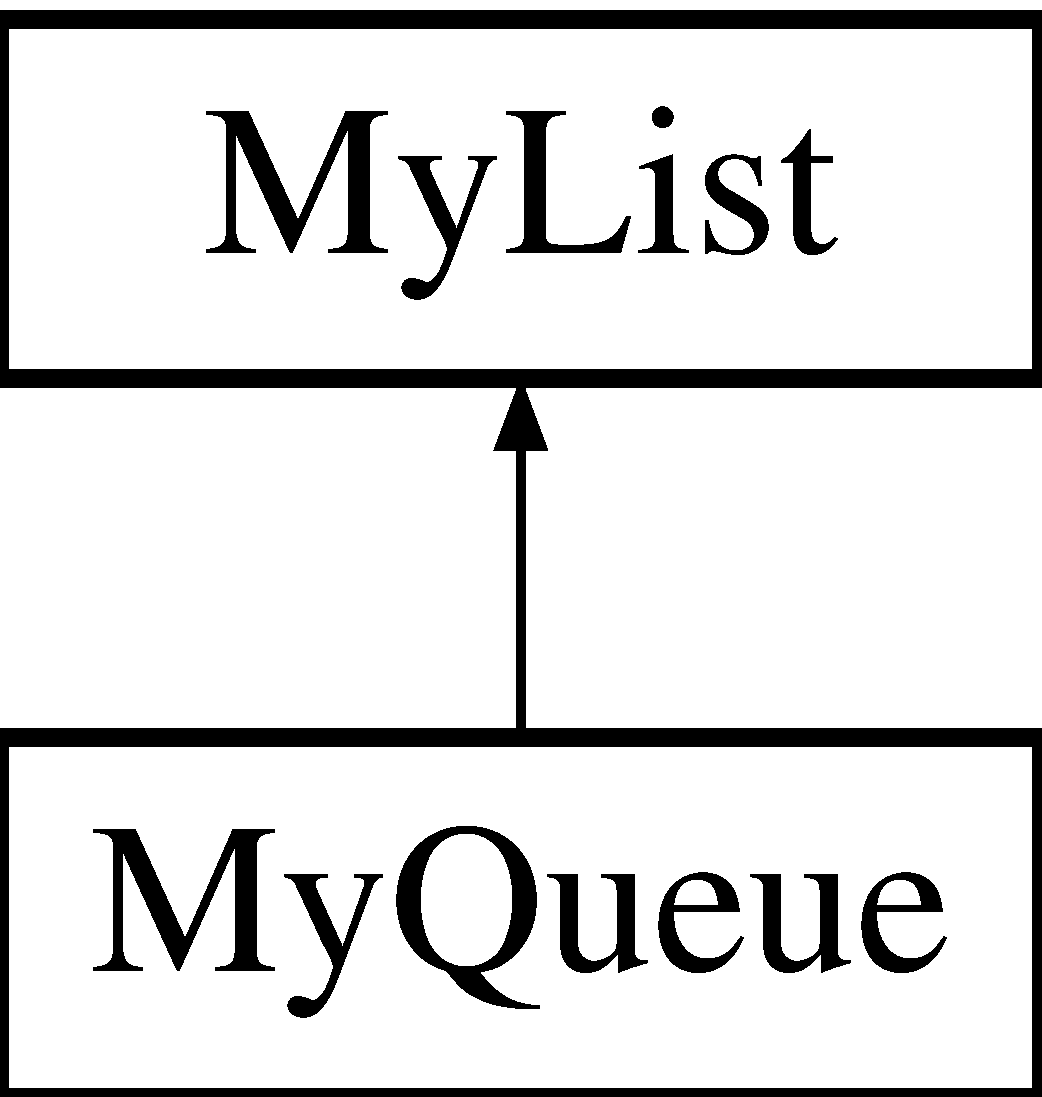
\includegraphics[height=2.000000cm]{class_my_queue}
\end{center}
\end{figure}
\subsubsection*{Metody publiczne}
\begin{DoxyCompactItemize}
\item 
void \hyperlink{class_my_queue_abc623d6dea3f8ea4c364d4e755914b89}{push} (int arg)
\item 
int \hyperlink{class_my_queue_a1515805489e2e6b4c955f8e1e62a0650}{pop} ()
\begin{DoxyCompactList}\small\item\em Wyciaga element z kolejki. \end{DoxyCompactList}\end{DoxyCompactItemize}


\subsubsection{Opis szczegółowy}


Definicja w linii \hyperlink{myqueue_8h_source_l00016}{16} pliku \hyperlink{myqueue_8h_source}{myqueue.\-h}.



\subsubsection{Dokumentacja funkcji składowych}
\hypertarget{class_my_queue_a1515805489e2e6b4c955f8e1e62a0650}{\index{My\-Queue@{My\-Queue}!pop@{pop}}
\index{pop@{pop}!MyQueue@{My\-Queue}}
\paragraph[{pop}]{\setlength{\rightskip}{0pt plus 5cm}int My\-Queue\-::pop (
\begin{DoxyParamCaption}
{}
\end{DoxyParamCaption}
)\hspace{0.3cm}{\ttfamily [inline]}}}\label{class_my_queue_a1515805489e2e6b4c955f8e1e62a0650}


Definicja w linii \hyperlink{myqueue_8h_source_l00027}{27} pliku \hyperlink{myqueue_8h_source}{myqueue.\-h}.



Odwołuje się do \hyperlink{mylist_8cpp_source_l00046}{My\-List\-::pop\-\_\-front()}.



Odwołania w \hyperlink{main_8cpp_source_l00017}{main()}.


\begin{DoxyCode}
00027                   \{
00028                 \textcolor{keywordflow}{return} \hyperlink{class_my_list_ae038b14e6cb5b54b8499b85ce5f03a0e}{pop\_front}();
00029         \}
\end{DoxyCode}
\hypertarget{class_my_queue_abc623d6dea3f8ea4c364d4e755914b89}{\index{My\-Queue@{My\-Queue}!push@{push}}
\index{push@{push}!MyQueue@{My\-Queue}}
\paragraph[{push}]{\setlength{\rightskip}{0pt plus 5cm}void My\-Queue\-::push (
\begin{DoxyParamCaption}
\item[{int}]{arg}
\end{DoxyParamCaption}
)\hspace{0.3cm}{\ttfamily [inline]}}}\label{class_my_queue_abc623d6dea3f8ea4c364d4e755914b89}


Definicja w linii \hyperlink{myqueue_8h_source_l00023}{23} pliku \hyperlink{myqueue_8h_source}{myqueue.\-h}.



Odwołuje się do \hyperlink{mylist_8cpp_source_l00018}{My\-List\-::push\-\_\-back()}.



Odwołania w \hyperlink{main_8cpp_source_l00017}{main()}.


\begin{DoxyCode}
00023                            \{
00024                 \hyperlink{class_my_list_a8428cca9d08fcf02e378aee0a232e971}{push\_back}(arg);
00025         \}
\end{DoxyCode}


Dokumentacja dla tej klasy została wygenerowana z pliku\-:\begin{DoxyCompactItemize}
\item 
\hyperlink{myqueue_8h}{myqueue.\-h}\end{DoxyCompactItemize}

\hypertarget{class_my_stack}{\subsection{Dokumentacja klasy My\-Stack}
\label{class_my_stack}\index{My\-Stack@{My\-Stack}}
}


Klasa reprezentuje stos.  




{\ttfamily \#include $<$mystack.\-h$>$}

Diagram dziedziczenia dla My\-Stack\begin{figure}[H]
\begin{center}
\leavevmode
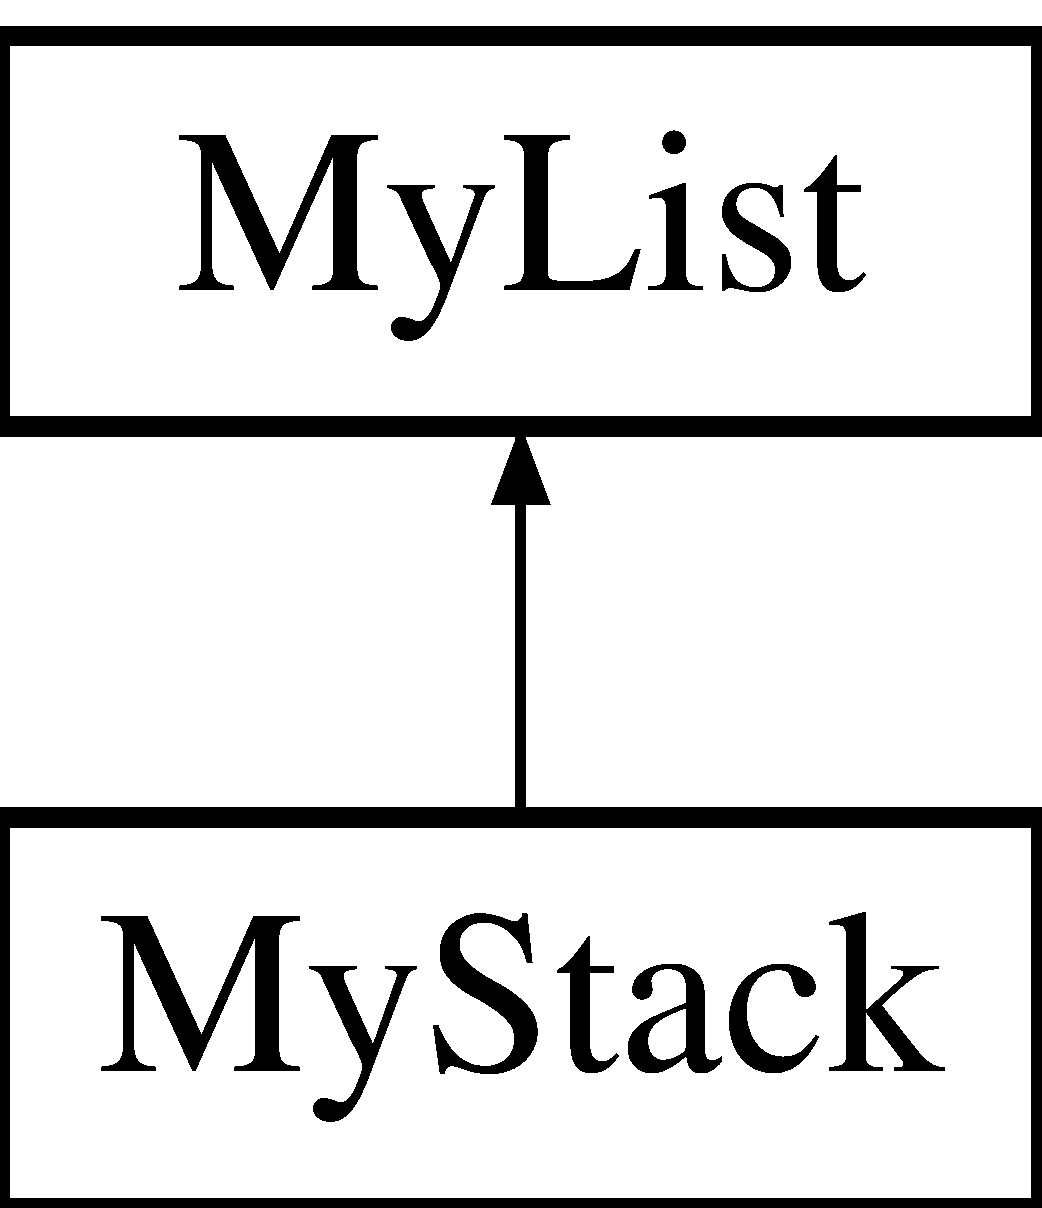
\includegraphics[height=2.000000cm]{class_my_stack}
\end{center}
\end{figure}
\subsubsection*{Metody publiczne}
\begin{DoxyCompactItemize}
\item 
void \hyperlink{class_my_stack_a481713bcbaecb7509a8903911db89331}{push} (int arg)
\item 
int \hyperlink{class_my_stack_abe5267f1fbc044957e8eb2e87fd10ca1}{pop} ()
\begin{DoxyCompactList}\small\item\em Wyciaga element ze stosu. \end{DoxyCompactList}\end{DoxyCompactItemize}


\subsubsection{Opis szczegółowy}
Stos, którego index po pushu pokazuje na miejsce nastepne(nastepne za tym elementem) 

Definicja w linii \hyperlink{mystack_8h_source_l00018}{18} pliku \hyperlink{mystack_8h_source}{mystack.\-h}.



\subsubsection{Dokumentacja funkcji składowych}
\hypertarget{class_my_stack_abe5267f1fbc044957e8eb2e87fd10ca1}{\index{My\-Stack@{My\-Stack}!pop@{pop}}
\index{pop@{pop}!MyStack@{My\-Stack}}
\paragraph[{pop}]{\setlength{\rightskip}{0pt plus 5cm}int My\-Stack\-::pop (
\begin{DoxyParamCaption}
{}
\end{DoxyParamCaption}
)\hspace{0.3cm}{\ttfamily [inline]}}}\label{class_my_stack_abe5267f1fbc044957e8eb2e87fd10ca1}


Definicja w linii \hyperlink{mystack_8h_source_l00029}{29} pliku \hyperlink{mystack_8h_source}{mystack.\-h}.



Odwołuje się do \hyperlink{mylist_8cpp_source_l00037}{My\-List\-::pop\-\_\-back()}.


\begin{DoxyCode}
00029                   \{
00030                 \textcolor{keywordflow}{return} \hyperlink{class_my_list_a7361ad3b0da0402cb95adb225ebfaffd}{pop\_back}();
00031         \}
\end{DoxyCode}
\hypertarget{class_my_stack_a481713bcbaecb7509a8903911db89331}{\index{My\-Stack@{My\-Stack}!push@{push}}
\index{push@{push}!MyStack@{My\-Stack}}
\paragraph[{push}]{\setlength{\rightskip}{0pt plus 5cm}void My\-Stack\-::push (
\begin{DoxyParamCaption}
\item[{int}]{arg}
\end{DoxyParamCaption}
)\hspace{0.3cm}{\ttfamily [inline]}}}\label{class_my_stack_a481713bcbaecb7509a8903911db89331}


Definicja w linii \hyperlink{mystack_8h_source_l00025}{25} pliku \hyperlink{mystack_8h_source}{mystack.\-h}.



Odwołuje się do \hyperlink{mylist_8cpp_source_l00018}{My\-List\-::push\-\_\-back()}.


\begin{DoxyCode}
00025                            \{
00026                 \hyperlink{class_my_list_a8428cca9d08fcf02e378aee0a232e971}{push\_back}(arg);
00027         \}
\end{DoxyCode}


Dokumentacja dla tej klasy została wygenerowana z pliku\-:\begin{DoxyCompactItemize}
\item 
\hyperlink{mystack_8h}{mystack.\-h}\end{DoxyCompactItemize}

\hypertarget{class_number_generator}{\subsection{Dokumentacja klasy Number\-Generator}
\label{class_number_generator}\index{Number\-Generator@{Number\-Generator}}
}


Klasa generujaca losowe liczby.  




{\ttfamily \#include $<$numbergenerator.\-h$>$}

Diagram dziedziczenia dla Number\-Generator\begin{figure}[H]
\begin{center}
\leavevmode
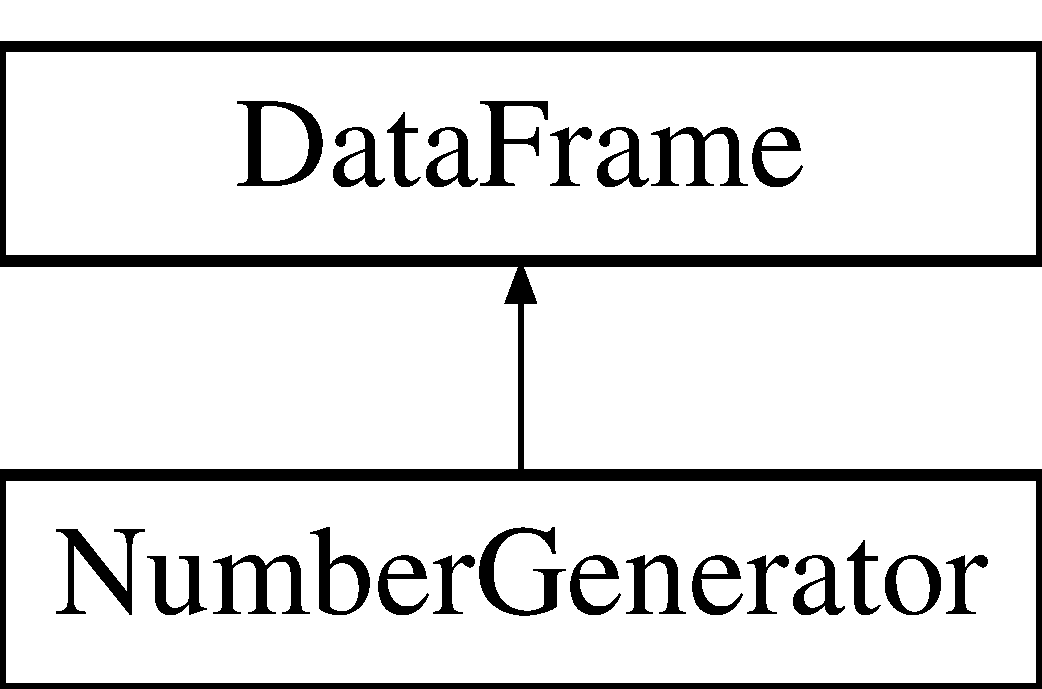
\includegraphics[height=2.000000cm]{class_number_generator}
\end{center}
\end{figure}
\subsubsection*{Metody publiczne}
\begin{DoxyCompactItemize}
\item 
void \hyperlink{class_number_generator_afe038fce2f1a2c90847fd483beea0494}{generate\-Numbers} ()
\begin{DoxyCompactList}\small\item\em Generuje losowe liczby. \end{DoxyCompactList}\item 
\hyperlink{class_number_generator_a828757cc2c9712e0b111584d1f1d5164}{$\sim$\-Number\-Generator} ()
\end{DoxyCompactItemize}
\subsubsection*{Dodatkowe Dziedziczone Składowe}


\subsubsection{Opis szczegółowy}
Klasa generujaca losowe liczby na podstawie czasu maszyny na ktorym jest uruchomiona Wszystkie funkcje zapisu pliku dziedziczy z klasy \hyperlink{class_data_frame}{Data\-Frame} 

Definicja w linii \hyperlink{numbergenerator_8h_source_l00023}{23} pliku \hyperlink{numbergenerator_8h_source}{numbergenerator.\-h}.



\subsubsection{Dokumentacja konstruktora i destruktora}
\hypertarget{class_number_generator_a828757cc2c9712e0b111584d1f1d5164}{\index{Number\-Generator@{Number\-Generator}!$\sim$\-Number\-Generator@{$\sim$\-Number\-Generator}}
\index{$\sim$\-Number\-Generator@{$\sim$\-Number\-Generator}!NumberGenerator@{Number\-Generator}}
\paragraph[{$\sim$\-Number\-Generator}]{\setlength{\rightskip}{0pt plus 5cm}Number\-Generator\-::$\sim$\-Number\-Generator (
\begin{DoxyParamCaption}
{}
\end{DoxyParamCaption}
)\hspace{0.3cm}{\ttfamily [inline]}}}\label{class_number_generator_a828757cc2c9712e0b111584d1f1d5164}


Definicja w linii \hyperlink{numbergenerator_8h_source_l00044}{44} pliku \hyperlink{numbergenerator_8h_source}{numbergenerator.\-h}.


\begin{DoxyCode}
00044 \{\}
\end{DoxyCode}


\subsubsection{Dokumentacja funkcji składowych}
\hypertarget{class_number_generator_afe038fce2f1a2c90847fd483beea0494}{\index{Number\-Generator@{Number\-Generator}!generate\-Numbers@{generate\-Numbers}}
\index{generate\-Numbers@{generate\-Numbers}!NumberGenerator@{Number\-Generator}}
\paragraph[{generate\-Numbers}]{\setlength{\rightskip}{0pt plus 5cm}void Number\-Generator\-::generate\-Numbers (
\begin{DoxyParamCaption}
{}
\end{DoxyParamCaption}
)\hspace{0.3cm}{\ttfamily [inline]}}}\label{class_number_generator_afe038fce2f1a2c90847fd483beea0494}
Generuje losowe liczby na podstawie czasu maszyny 

Definicja w linii \hyperlink{numbergenerator_8h_source_l00031}{31} pliku \hyperlink{numbergenerator_8h_source}{numbergenerator.\-h}.



Odwołuje się do \hyperlink{dataframe_8h_source_l00034}{Data\-Frame\-::size\-Of\-Table} i \hyperlink{dataframe_8h_source_l00021}{Data\-Frame\-::table\-Of\-Data}.


\begin{DoxyCode}
00032 \{
00033         time\_t randomTime = clock();
00034         this->\hyperlink{class_data_frame_a8edc4ce524483e2e5069067267ccdcbf}{tableOfData} = \textcolor{keyword}{new} \textcolor{keywordtype}{int}[\hyperlink{class_data_frame_aa5d1905c6910cad07ab5189bd34b13ab}{sizeOfTable}];
00035         \textcolor{keywordflow}{for}(\textcolor{keywordtype}{unsigned} \textcolor{keywordtype}{int} i=0; i<\hyperlink{class_data_frame_aa5d1905c6910cad07ab5189bd34b13ab}{sizeOfTable} ; i++)
00036         \{
00037                 srand (randomTime = clock());
00038                 this->\hyperlink{class_data_frame_a8edc4ce524483e2e5069067267ccdcbf}{tableOfData}[i] = rand()%100;
00039                 randomTime = clock();
00040         \}
00041 \}
\end{DoxyCode}


Dokumentacja dla tej klasy została wygenerowana z pliku\-:\begin{DoxyCompactItemize}
\item 
\hyperlink{numbergenerator_8h}{numbergenerator.\-h}\end{DoxyCompactItemize}

\section{Dokumentacja plików}
\hypertarget{dataframe_8cpp}{\subsection{Dokumentacja pliku dataframe.\-cpp}
\label{dataframe_8cpp}\index{dataframe.\-cpp@{dataframe.\-cpp}}
}
{\ttfamily \#include \char`\"{}dataframe.\-h\char`\"{}}\\*

\hypertarget{dataframe_8cpp}{\subsection{dataframe.\-cpp}
\label{dataframe_8cpp}\index{dataframe.\-cpp@{dataframe.\-cpp}}
}

\begin{DoxyCode}
00001 \textcolor{comment}{/*}
00002 \textcolor{comment}{ * dataframe.cpp}
00003 \textcolor{comment}{ *}
00004 \textcolor{comment}{ *  Created on: Mar 7, 2015}
00005 \textcolor{comment}{ *      Author: serek8}
00006 \textcolor{comment}{ */}
00007 
00010 \textcolor{preprocessor}{#include "\hyperlink{dataframe_8h}{dataframe.h}"}
00011 
\hypertarget{dataframe_8cpp_source_l00012}{}\hyperlink{class_data_frame_a69a9dc47b7506b8062fd34aedacbf579}{00012} \hyperlink{class_data_frame_a69a9dc47b7506b8062fd34aedacbf579}{DataFrame::DataFrame}()
00013 \{
00014         \hyperlink{class_data_frame_a8edc4ce524483e2e5069067267ccdcbf}{tableOfData} = 0;
00015         \hyperlink{class_data_frame_a824a73f019aec71281837abafd95a510}{outputFileName} = NULL;
00016         \hyperlink{class_data_frame_a90041bfdf474b0d7ce39bc3dbbb55aa9}{inputFileName} = NULL;
00017         \hyperlink{class_data_frame_aa5d1905c6910cad07ab5189bd34b13ab}{sizeOfTable} = 0;
00018 \}
00019 
\hypertarget{dataframe_8cpp_source_l00020}{}\hyperlink{class_data_frame_a617ef21804065f31115c01527155f499}{00020} \textcolor{keywordtype}{int} \hyperlink{class_data_frame_a617ef21804065f31115c01527155f499}{DataFrame :: loadDataFromFile}()
00021 \{
00022         std::ifstream streamToFile;
00023         streamToFile.open (\hyperlink{class_data_frame_a90041bfdf474b0d7ce39bc3dbbb55aa9}{inputFileName}, std::ifstream::in);
00024         this->\hyperlink{class_data_frame_a8edc4ce524483e2e5069067267ccdcbf}{tableOfData} = \textcolor{keyword}{new} \textcolor{keywordtype}{int}[\hyperlink{class_data_frame_aa5d1905c6910cad07ab5189bd34b13ab}{sizeOfTable}];
00025         \textcolor{keywordflow}{for}(\textcolor{keywordtype}{unsigned} \textcolor{keywordtype}{int} i=0; i<\hyperlink{class_data_frame_aa5d1905c6910cad07ab5189bd34b13ab}{sizeOfTable} ; i++) \{
00026                 streamToFile >> this-> \hyperlink{class_data_frame_a8edc4ce524483e2e5069067267ccdcbf}{tableOfData}[i];
00027                 \textcolor{keywordflow}{if} (streamToFile.eof()) \textcolor{keywordflow}{return} 1; \textcolor{comment}{//[EoF reached]}
00028         \}
00029         \textcolor{keywordflow}{return} 0;
00030 \}
00031 
\hypertarget{dataframe_8cpp_source_l00032}{}\hyperlink{class_data_frame_a03cc3ac606fdb8a2dbcaea5d429cf208}{00032} \textcolor{keywordtype}{int} \hyperlink{class_data_frame_a03cc3ac606fdb8a2dbcaea5d429cf208}{DataFrame :: saveDataToFile}()
00033 \{
00034         std::ofstream streamToFile;
00035         streamToFile.open (\hyperlink{class_data_frame_a824a73f019aec71281837abafd95a510}{outputFileName}, std::ofstream::out);
00036         \textcolor{keywordflow}{for}(\textcolor{keywordtype}{unsigned} \textcolor{keywordtype}{int} i=0; i<\hyperlink{class_data_frame_aa5d1905c6910cad07ab5189bd34b13ab}{sizeOfTable} ; i++) \{
00037                 streamToFile << this-> \hyperlink{class_data_frame_a8edc4ce524483e2e5069067267ccdcbf}{tableOfData}[i] <<\textcolor{charliteral}{' '};
00038         \}
00039         \textcolor{keywordflow}{return} 0;
00040 \}
00041 
00042 
00043 
\hypertarget{dataframe_8cpp_source_l00044}{}\hyperlink{class_data_frame_ab7dddb09f5ee9dc4a5783136dad01962}{00044} \hyperlink{class_data_frame}{DataFrame} \hyperlink{class_data_frame_ab7dddb09f5ee9dc4a5783136dad01962}{DataFrame :: operator= }(\hyperlink{class_data_frame}{DataFrame} dataframe)
00045 \{
00046         this->\hyperlink{class_data_frame_a8edc4ce524483e2e5069067267ccdcbf}{tableOfData} = dataframe.\hyperlink{class_data_frame_a8edc4ce524483e2e5069067267ccdcbf}{tableOfData};
00047         this->\hyperlink{class_data_frame_a824a73f019aec71281837abafd95a510}{outputFileName} = dataframe.\hyperlink{class_data_frame_a824a73f019aec71281837abafd95a510}{outputFileName};
00048         this->\hyperlink{class_data_frame_a90041bfdf474b0d7ce39bc3dbbb55aa9}{inputFileName} = dataframe.\hyperlink{class_data_frame_a90041bfdf474b0d7ce39bc3dbbb55aa9}{inputFileName};
00049         this->\hyperlink{class_data_frame_aa5d1905c6910cad07ab5189bd34b13ab}{sizeOfTable} = dataframe.\hyperlink{class_data_frame_aa5d1905c6910cad07ab5189bd34b13ab}{sizeOfTable};
00050         \textcolor{keywordflow}{return} *\textcolor{keyword}{this};
00051 \}
\end{DoxyCode}

\hypertarget{dataframe_8h}{\section{Dokumentacja pliku dataframe.\-h}
\label{dataframe_8h}\index{dataframe.\-h@{dataframe.\-h}}
}
{\ttfamily \#include $<$fstream$>$}\\*
\subsection*{Komponenty}
\begin{DoxyCompactItemize}
\item 
class \hyperlink{class_data_frame}{Data\-Frame}
\end{DoxyCompactItemize}

\hypertarget{dataframe_8h}{\subsection{dataframe.\-h}
\label{dataframe_8h}\index{dataframe.\-h@{dataframe.\-h}}
}

\begin{DoxyCode}
00001 \textcolor{comment}{/*}
00002 \textcolor{comment}{ * dataframe.h}
00003 \textcolor{comment}{ *}
00004 \textcolor{comment}{ *  Created on: Mar 6, 2015}
00005 \textcolor{comment}{ *      Author: serek8}
00006 \textcolor{comment}{ */}
00008 \textcolor{preprocessor}{#ifndef DATAFRAME\_H\_}
00009 \textcolor{preprocessor}{}\textcolor{preprocessor}{#define DATAFRAME\_H\_}
00010 \textcolor{preprocessor}{}
00011 \textcolor{preprocessor}{#include <fstream>}
00012 
00013 
00014 
\hypertarget{dataframe_8h_source_l00015}{}\hyperlink{class_data_frame}{00015} \textcolor{keyword}{class }\hyperlink{class_data_frame}{DataFrame}
00016 \{
00017 \textcolor{keyword}{public}:
\hypertarget{dataframe_8h_source_l00021}{}\hyperlink{class_data_frame_a8edc4ce524483e2e5069067267ccdcbf}{00021}         \textcolor{keywordtype}{int} *\hyperlink{class_data_frame_a8edc4ce524483e2e5069067267ccdcbf}{tableOfData};
\hypertarget{dataframe_8h_source_l00025}{}\hyperlink{class_data_frame_a824a73f019aec71281837abafd95a510}{00025}         \textcolor{keywordtype}{char} *\hyperlink{class_data_frame_a824a73f019aec71281837abafd95a510}{outputFileName};
\hypertarget{dataframe_8h_source_l00029}{}\hyperlink{class_data_frame_a90041bfdf474b0d7ce39bc3dbbb55aa9}{00029}         \textcolor{keywordtype}{char} *\hyperlink{class_data_frame_a90041bfdf474b0d7ce39bc3dbbb55aa9}{inputFileName};
\hypertarget{dataframe_8h_source_l00034}{}\hyperlink{class_data_frame_aa5d1905c6910cad07ab5189bd34b13ab}{00034}         \textcolor{keywordtype}{unsigned} \textcolor{keywordtype}{int} \hyperlink{class_data_frame_aa5d1905c6910cad07ab5189bd34b13ab}{sizeOfTable};
00035 
00039         \hyperlink{class_data_frame_a69a9dc47b7506b8062fd34aedacbf579}{DataFrame}();
00049         \textcolor{keywordtype}{int} \hyperlink{class_data_frame_a617ef21804065f31115c01527155f499}{loadDataFromFile}();
00050 
00056         \textcolor{keywordtype}{int} \hyperlink{class_data_frame_a03cc3ac606fdb8a2dbcaea5d429cf208}{saveDataToFile}();
00057 
00063         \hyperlink{class_data_frame}{DataFrame} \hyperlink{class_data_frame_ab7dddb09f5ee9dc4a5783136dad01962}{operator= }(\hyperlink{class_data_frame}{DataFrame} dataframe);
\hypertarget{dataframe_8h_source_l00064}{}\hyperlink{class_data_frame_a1360ddf00d717392fe1292bc1e1990ff}{00064}         \textcolor{keyword}{virtual} \hyperlink{class_data_frame_a1360ddf00d717392fe1292bc1e1990ff}{~DataFrame}() \{\}
00065 
00066 
00067 \};
00068 
00069 
00070 
00071 \textcolor{preprocessor}{#endif }\textcolor{comment}{/* DATAFRAME\_H\_ */}\textcolor{preprocessor}{}
\end{DoxyCode}

\hypertarget{main_8cpp}{\subsection{Dokumentacja pliku main.\-cpp}
\label{main_8cpp}\index{main.\-cpp@{main.\-cpp}}
}
{\ttfamily \#include $<$iostream$>$}\\*
{\ttfamily \#include $<$unistd.\-h$>$}\\*
{\ttfamily \#include \char`\"{}multiplybytwo.\-h\char`\"{}}\\*
{\ttfamily \#include \char`\"{}numbergenerator.\-h\char`\"{}}\\*
{\ttfamily \#include \char`\"{}dataframe.\-h\char`\"{}}\\*
{\ttfamily \#include \char`\"{}mystack.\-h\char`\"{}}\\*
{\ttfamily \#include \char`\"{}myqueue.\-h\char`\"{}}\\*
\subsubsection*{Funkcje}
\begin{DoxyCompactItemize}
\item 
int \hyperlink{main_8cpp_a0ddf1224851353fc92bfbff6f499fa97}{main} (int argc, char $\ast$argv\mbox{[}$\,$\mbox{]})
\end{DoxyCompactItemize}


\subsubsection{Dokumentacja funkcji}
\hypertarget{main_8cpp_a0ddf1224851353fc92bfbff6f499fa97}{\index{main.\-cpp@{main.\-cpp}!main@{main}}
\index{main@{main}!main.cpp@{main.\-cpp}}
\paragraph[{main}]{\setlength{\rightskip}{0pt plus 5cm}int main (
\begin{DoxyParamCaption}
\item[{int}]{argc, }
\item[{char $\ast$}]{argv\mbox{[}$\,$\mbox{]}}
\end{DoxyParamCaption}
)}}\label{main_8cpp_a0ddf1224851353fc92bfbff6f499fa97}
Ilosc powtorzen przez algorytmu

Zmienna uzywana przez G\-E\-T\-O\-P\-T

Flaga ktora mowi o tym czy wlaczyc generator liczb losowych

Czesc testowa programu

Definicja w linii \hyperlink{main_8cpp_source_l00017}{17} pliku \hyperlink{main_8cpp_source}{main.\-cpp}.



Odwołuje się do \hyperlink{multiplybytwo_8cpp_source_l00011}{Multiply\-By\-Two\-::execute\-Algorithm()}, \hyperlink{numbergenerator_8h_source_l00031}{Number\-Generator\-::generate\-Numbers()}, \hyperlink{dataframe_8h_source_l00029}{Data\-Frame\-::input\-File\-Name}, \hyperlink{dataframe_8cpp_source_l00020}{Data\-Frame\-::load\-Data\-From\-File()}, \hyperlink{dataframe_8h_source_l00025}{Data\-Frame\-::output\-File\-Name}, \hyperlink{myqueue_8h_source_l00027}{My\-Queue\-::pop()}, \hyperlink{myqueue_8h_source_l00023}{My\-Queue\-::push()}, \hyperlink{dataframe_8cpp_source_l00032}{Data\-Frame\-::save\-Data\-To\-File()}, \hyperlink{dataframe_8h_source_l00034}{Data\-Frame\-::size\-Of\-Table} i \hyperlink{mybenchmark_8cpp_source_l00012}{My\-Benchmark\-::test\-Algorithm()}.


\begin{DoxyCode}
00018 \{
00019         \hyperlink{class_data_frame}{DataFrame} podstawoweInfoIO;
00020         \textcolor{keywordtype}{int} quantityRepetitionOfAlgorithm = 0;  
00021 
00022         \textcolor{keywordtype}{int} opt;        
00023         \textcolor{keywordtype}{bool} isSetNumberGenerator=\textcolor{keyword}{false}; 
00024         \textcolor{keywordtype}{bool} isTest=\textcolor{keyword}{false};
00025 
00026         \textcolor{keywordflow}{while} ((opt = getopt(argc, argv, \textcolor{stringliteral}{"n:t:o:i:gx"})) != -1) \{
00027                 \textcolor{keywordflow}{switch}(opt)\{
00028                 \textcolor{keywordflow}{case} \textcolor{charliteral}{'n'}:       \textcolor{comment}{// ilosc liczb do przetworzenia}
00029                         podstawoweInfoIO.\hyperlink{class_data_frame_aa5d1905c6910cad07ab5189bd34b13ab}{sizeOfTable} = atoi(optarg);
00030                         \textcolor{keywordflow}{break};
00031 
00032                 \textcolor{keywordflow}{case} \textcolor{charliteral}{'t'}:       \textcolor{comment}{// wlacza benchmark i przyjmuje liczbe powtorzen dla benchmarka}
00033                         quantityRepetitionOfAlgorithm = atoi(optarg);
00034                         \textcolor{keywordflow}{break};
00035 
00036                 \textcolor{keywordflow}{case} \textcolor{charliteral}{'o'}:
00037                         podstawoweInfoIO.\hyperlink{class_data_frame_a824a73f019aec71281837abafd95a510}{outputFileName} = optarg;
00038                         \textcolor{keywordflow}{break};
00039 
00040                 \textcolor{keywordflow}{case} \textcolor{charliteral}{'i'}:
00041                         podstawoweInfoIO.\hyperlink{class_data_frame_a90041bfdf474b0d7ce39bc3dbbb55aa9}{inputFileName}=optarg;
00042                         \textcolor{keywordflow}{break};
00043 
00044                 \textcolor{keywordflow}{case} \textcolor{charliteral}{'g'}:       \textcolor{comment}{// wlacza generator liczb, po zakonczeniu generowania konczy program}
00045                         isSetNumberGenerator=\textcolor{keyword}{true};
00046                         \textcolor{keywordflow}{break};
00047 
00048                 \textcolor{keywordflow}{case} \textcolor{charliteral}{'x'}:       \textcolor{comment}{// miejsce dla programisty dla sprawdzania kodu}
00049                         isTest =1;
00050                         \textcolor{keywordflow}{break};
00051 
00052                 \textcolor{keywordflow}{case} \textcolor{charliteral}{'?'}:
00053                 \textcolor{keywordflow}{default}:
00054                         std::cout<<\textcolor{stringliteral}{"\(\backslash\)nPodano zly argument"};
00055                         \textcolor{keywordflow}{return} -1;
00056                 \}
00057         \}
00061         \textcolor{keywordflow}{if}(isTest)
00062         \{
00063                 \hyperlink{class_my_queue}{MyQueue} stack;
00064                 stack.\hyperlink{class_my_queue_abc623d6dea3f8ea4c364d4e755914b89}{push}(1); stack.\hyperlink{class_my_queue_abc623d6dea3f8ea4c364d4e755914b89}{push}(2); stack.\hyperlink{class_my_queue_abc623d6dea3f8ea4c364d4e755914b89}{push}(3);
00065                 std::cout<<stack.\hyperlink{class_my_queue_a1515805489e2e6b4c955f8e1e62a0650}{pop}();
00066                 std::cout<<stack.\hyperlink{class_my_queue_a1515805489e2e6b4c955f8e1e62a0650}{pop}();
00067                 std::cout<<stack.\hyperlink{class_my_queue_a1515805489e2e6b4c955f8e1e62a0650}{pop}();
00068                 \textcolor{keywordflow}{return} 0;
00069         \}
00070 
00071 
00072         \textcolor{comment}{/*}
00073 \textcolor{comment}{         * Sprawdzam czy program zostal uzyty tylko do wygenerowania liczb losowych}
00074 \textcolor{comment}{         * jesli tak to tworze te liczby zgodnie quantityNumber i zamykam program}
00075 \textcolor{comment}{         */}
00076         \textcolor{keywordflow}{if}(isSetNumberGenerator) \{
00077         \hyperlink{class_number_generator}{NumberGenerator} generator;
00078         generator= podstawoweInfoIO;
00079         generator.\hyperlink{class_number_generator_afe038fce2f1a2c90847fd483beea0494}{generateNumbers}();
00080         generator.\hyperlink{class_data_frame_a03cc3ac606fdb8a2dbcaea5d429cf208}{saveDataToFile}();
00081         std::cout<<\textcolor{stringliteral}{"\(\backslash\)nZapisane.\(\backslash\)n"};
00082         \textcolor{keywordflow}{return} 0;
00083         \}
00084 
00085 
00086         \hyperlink{class_multiply_by_two}{MultiplyByTwo} algorytm\_x2 ;
00087         algorytm\_x2= podstawoweInfoIO;
00088 
00089         \textcolor{comment}{/*}
00090 \textcolor{comment}{         *  Wczytuje liczby z pliku do przeprowadzenia algorytmu}
00091 \textcolor{comment}{         */}
00092         \textcolor{keywordflow}{if}(algorytm\_x2.\hyperlink{class_data_frame_a617ef21804065f31115c01527155f499}{loadDataFromFile}()) \{
00093                 std::cout<<\textcolor{stringliteral}{"\(\backslash\)nNie istnieje tyle liczb w pliku !\(\backslash\)nKoncze program"};
00094                 \textcolor{keywordflow}{return} 1;
00095         \}
00096 
00097         \textcolor{comment}{/*}
00098 \textcolor{comment}{         * Sprawdzam czy otrzymalem agrument o testowaniu algorytmu,}
00099 \textcolor{comment}{         * a nastepnie przeprawadzam test albo uruchamiam normalnie algorytm}
00100 \textcolor{comment}{         */}
00101         \textcolor{keywordflow}{if}(quantityRepetitionOfAlgorithm)\{
00102                 std::cout<<\textcolor{stringliteral}{"\(\backslash\)nCzas algorytmu: "}<<algorytm\_x2.\hyperlink{class_my_benchmark_a66576625ca37f8bc539c18ffceb69c9c}{testAlgorithm}(
      quantityRepetitionOfAlgorithm)<<\textcolor{charliteral}{'\(\backslash\)n'};
00103         \}
00104         \textcolor{keywordflow}{else} \{
00105                 algorytm\_x2.\hyperlink{class_multiply_by_two_aad2080a1fdab088814170e529a14db1e}{executeAlgorithm}();
00106         \}
00107 
00108         \textcolor{comment}{/*}
00109 \textcolor{comment}{         * Zapisuje wyniki do pliku}
00110 \textcolor{comment}{         */}
00111         algorytm\_x2.\hyperlink{class_data_frame_a03cc3ac606fdb8a2dbcaea5d429cf208}{saveDataToFile}();
00112 
00113         \textcolor{keywordflow}{return} 0;
00114 \}
\end{DoxyCode}

\hypertarget{main_8cpp}{\subsection{main.\-cpp}
\label{main_8cpp}\index{main.\-cpp@{main.\-cpp}}
}

\begin{DoxyCode}
00001 \textcolor{comment}{/*}
00002 \textcolor{comment}{ * main.cpp}
00003 \textcolor{comment}{ *}
00004 \textcolor{comment}{ *  Created on: Mar 6, 2015}
00005 \textcolor{comment}{ *      Author: serek8}
00006 \textcolor{comment}{ */}
00008 \textcolor{preprocessor}{#include <iostream>}
00009 \textcolor{preprocessor}{#include <unistd.h>}
00010 \textcolor{preprocessor}{#include <stdlib.h>}
00011 \textcolor{preprocessor}{#include "\hyperlink{multiplybytwo_8h}{multiplybytwo.h}"}
00012 \textcolor{preprocessor}{#include "\hyperlink{numbergenerator_8h}{numbergenerator.h}"}
00013 \textcolor{preprocessor}{#include "\hyperlink{dataframe_8h}{dataframe.h}"}
00014 
00015 
\hypertarget{main_8cpp_source_l00016}{}\hyperlink{main_8cpp_a0ddf1224851353fc92bfbff6f499fa97}{00016} \textcolor{keywordtype}{int} \hyperlink{main_8cpp_a0ddf1224851353fc92bfbff6f499fa97}{main}(\textcolor{keywordtype}{int} argc, \textcolor{keywordtype}{char} *argv[])
00017 \{
00018         \hyperlink{class_data_frame}{DataFrame} podstawoweInfoIO;
00019         \textcolor{keywordtype}{int} quantityRepetitionOfAlgorithm = 0;  
00020 
00021         \textcolor{keywordtype}{int} opt;        
00022         \textcolor{keywordtype}{bool} isSetNumberGenerator=\textcolor{keyword}{false}; 
00023 
00024         \textcolor{keywordflow}{while} ((opt = getopt(argc, argv, \textcolor{stringliteral}{"n:t:o:i:g"})) != -1) \{
00025                 \textcolor{keywordflow}{switch}(opt)\{
00026                 \textcolor{keywordflow}{case} \textcolor{charliteral}{'n'}:
00027                         podstawoweInfoIO.\hyperlink{class_data_frame_aa5d1905c6910cad07ab5189bd34b13ab}{sizeOfTable} = atoi(optarg);
00028                         \textcolor{keywordflow}{break};
00029 
00030                 \textcolor{keywordflow}{case} \textcolor{charliteral}{'t'}:
00031                         quantityRepetitionOfAlgorithm = atoi(optarg);
00032                         \textcolor{keywordflow}{break};
00033 
00034                 \textcolor{keywordflow}{case} \textcolor{charliteral}{'o'}:
00035                         podstawoweInfoIO.\hyperlink{class_data_frame_a824a73f019aec71281837abafd95a510}{outputFileName} = optarg;
00036                         \textcolor{keywordflow}{break};
00037 
00038                 \textcolor{keywordflow}{case} \textcolor{charliteral}{'i'}:
00039                         podstawoweInfoIO.\hyperlink{class_data_frame_a90041bfdf474b0d7ce39bc3dbbb55aa9}{inputFileName}=optarg;
00040                         \textcolor{keywordflow}{break};
00041 
00042                 \textcolor{keywordflow}{case} \textcolor{charliteral}{'g'}:
00043                         isSetNumberGenerator=\textcolor{keyword}{true};
00044                         \textcolor{keywordflow}{break};
00045 
00046                 \textcolor{keywordflow}{case} \textcolor{charliteral}{'?'}:
00047                 \textcolor{keywordflow}{default}:
00048                         std::cout<<\textcolor{stringliteral}{"\(\backslash\)nPodano zly argument"};
00049                         \textcolor{keywordflow}{return} -1;
00050 
00051                 \}
00052         \}
00053         \textcolor{comment}{/*}
00054 \textcolor{comment}{         * Sprawdzam czy program zostal uzyty tylko do wygenerowania liczb losowych}
00055 \textcolor{comment}{         * jesli tak to tworze te liczby zgodnie quantityNumber i zamykam program}
00056 \textcolor{comment}{         */}
00057         \textcolor{keywordflow}{if}(isSetNumberGenerator) \{
00058         \hyperlink{class_number_generator}{NumberGenerator} generator;
00059         generator= podstawoweInfoIO;
00060         generator.\hyperlink{class_number_generator_afe038fce2f1a2c90847fd483beea0494}{generateNumbers}();
00061         generator.\hyperlink{class_data_frame_a03cc3ac606fdb8a2dbcaea5d429cf208}{saveDataToFile}();
00062         std::cout<<\textcolor{stringliteral}{"\(\backslash\)nZapisane.\(\backslash\)n"};
00063         \textcolor{keywordflow}{return} 0;
00064         \}
00065 
00066 
00067         \hyperlink{class_multiply_by_two}{MultiplyByTwo} algorytm\_x2 ;
00068         algorytm\_x2= podstawoweInfoIO;
00069 
00070         \textcolor{comment}{// Laduje liczby do przeprowadzenia algorytmu}
00071         \textcolor{keywordflow}{if}(algorytm\_x2.\hyperlink{class_data_frame_a617ef21804065f31115c01527155f499}{loadDataFromFile}()) \{
00072                 std::cout<<\textcolor{stringliteral}{"\(\backslash\)nNie istnieje tyle liczb w pliku !\(\backslash\)nKoncze program"};
00073                 \textcolor{keywordflow}{return} 1;
00074         \}
00075 
00076         \textcolor{comment}{/*}
00077 \textcolor{comment}{         * Sprawdzam czy otrzymalem agrument o testowaniu algorytmu,}
00078 \textcolor{comment}{         * a nastepnie przeprawadzam test albo uruchamiam normalnie algorytm}
00079 \textcolor{comment}{         */}
00080         \textcolor{keywordflow}{if}(quantityRepetitionOfAlgorithm)\{
00081                 std::cout<<\textcolor{stringliteral}{"\(\backslash\)nCzas algorytmu: "}<<algorytm\_x2.\hyperlink{class_my_benchmark_a66576625ca37f8bc539c18ffceb69c9c}{testAlgorithm}(
      quantityRepetitionOfAlgorithm)<<\textcolor{charliteral}{'\(\backslash\)n'};
00082         \}
00083         \textcolor{keywordflow}{else} \{
00084                 algorytm\_x2.\hyperlink{class_multiply_by_two_aad2080a1fdab088814170e529a14db1e}{executeAlgorithm}();
00085         \}
00086 
00087 
00088 
00089         algorytm\_x2.\hyperlink{class_data_frame_a03cc3ac606fdb8a2dbcaea5d429cf208}{saveDataToFile}();
00090 
00091         \textcolor{keywordflow}{return} 0;
00092 \}
\end{DoxyCode}

\hypertarget{multiplybytwo_8cpp}{\section{Dokumentacja pliku multiplybytwo.\-cpp}
\label{multiplybytwo_8cpp}\index{multiplybytwo.\-cpp@{multiplybytwo.\-cpp}}
}
{\ttfamily \#include \char`\"{}multiplybytwo.\-h\char`\"{}}\\*

\hypertarget{multiplybytwo_8cpp}{\subsection{multiplybytwo.\-cpp}
\label{multiplybytwo_8cpp}\index{multiplybytwo.\-cpp@{multiplybytwo.\-cpp}}
}

\begin{DoxyCode}
00001 \textcolor{comment}{/*}
00002 \textcolor{comment}{ * multiplybytwo.cpp}
00003 \textcolor{comment}{ *}
00004 \textcolor{comment}{ *  Created on: Mar 7, 2015}
00005 \textcolor{comment}{ *      Author: serek8}
00006 \textcolor{comment}{ */}
00009 \textcolor{preprocessor}{#include "\hyperlink{multiplybytwo_8h}{multiplybytwo.h}"}
00010 
\hypertarget{multiplybytwo_8cpp_source_l00011}{}\hyperlink{class_multiply_by_two_aad2080a1fdab088814170e529a14db1e}{00011} \textcolor{keywordtype}{void} \hyperlink{class_multiply_by_two_aad2080a1fdab088814170e529a14db1e}{MultiplyByTwo :: executeAlgorithm}()
00012 \{
00013         \textcolor{keywordflow}{for}(\textcolor{keywordtype}{unsigned} \textcolor{keywordtype}{int} i=0; i<\hyperlink{class_data_frame_aa5d1905c6910cad07ab5189bd34b13ab}{sizeOfTable}; i++) \{
00014 
00015                 \hyperlink{class_data_frame_a8edc4ce524483e2e5069067267ccdcbf}{tableOfData}[i]*=2;
00016         \}
00017 
00018 
00019 
00020 \}
00021 
00022 
\end{DoxyCode}

\hypertarget{multiplybytwo_8h}{\subsection{Dokumentacja pliku multiplybytwo.\-h}
\label{multiplybytwo_8h}\index{multiplybytwo.\-h@{multiplybytwo.\-h}}
}
{\ttfamily \#include \char`\"{}mybenchmark.\-h\char`\"{}}\\*
{\ttfamily \#include \char`\"{}dataframe.\-h\char`\"{}}\\*
\subsubsection*{Komponenty}
\begin{DoxyCompactItemize}
\item 
class \hyperlink{class_multiply_by_two}{Multiply\-By\-Two}
\begin{DoxyCompactList}\small\item\em Algorytm mnozy kazda liczbe razy 2. \end{DoxyCompactList}\end{DoxyCompactItemize}

\hypertarget{multiplybytwo_8h}{\subsection{multiplybytwo.\-h}
\label{multiplybytwo_8h}\index{multiplybytwo.\-h@{multiplybytwo.\-h}}
}

\begin{DoxyCode}
00001 \textcolor{comment}{/*}
00002 \textcolor{comment}{ * multiplybytwo.h}
00003 \textcolor{comment}{ *}
00004 \textcolor{comment}{ *  Created on: Mar 6, 2015}
00005 \textcolor{comment}{ *      Author: serek8}
00006 \textcolor{comment}{ */}
00008 \textcolor{preprocessor}{#ifndef MULTIPLYBYTWO\_H\_}
00009 \textcolor{preprocessor}{}\textcolor{preprocessor}{#define MULTIPLYBYTWO\_H\_}
00010 \textcolor{preprocessor}{}
00011 \textcolor{preprocessor}{#include "\hyperlink{mybenchmark_8h}{mybenchmark.h}"}
00012 \textcolor{preprocessor}{#include "\hyperlink{dataframe_8h}{dataframe.h}"}
00013 
00014 
\hypertarget{multiplybytwo_8h_source_l00020}{}\hyperlink{class_multiply_by_two}{00020} \textcolor{keyword}{class }\hyperlink{class_multiply_by_two}{MultiplyByTwo} : \textcolor{keyword}{public}  \hyperlink{class_my_benchmark}{MyBenchmark}
00021 \{
00022 \textcolor{keyword}{public}:
00027         \textcolor{keywordtype}{void} \hyperlink{class_multiply_by_two_aad2080a1fdab088814170e529a14db1e}{executeAlgorithm}();
00028 
\hypertarget{multiplybytwo_8h_source_l00029}{}\hyperlink{class_multiply_by_two_ab84d2c946e0ac7d6eeef32d5800ce4a5}{00029}         \hyperlink{class_multiply_by_two_ab84d2c946e0ac7d6eeef32d5800ce4a5}{~MultiplyByTwo}()\{\}
00030 
00031 
00032 
00033         \textcolor{keyword}{using} DataFrame::operator=;
00034 
00035 \};
00036 
00037 \textcolor{preprocessor}{#endif }\textcolor{comment}{/* MULTIPLYBYTWO\_H\_ */}\textcolor{preprocessor}{}
\end{DoxyCode}

\hypertarget{mybenchmark_8cpp}{\section{Dokumentacja pliku mybenchmark.\-cpp}
\label{mybenchmark_8cpp}\index{mybenchmark.\-cpp@{mybenchmark.\-cpp}}
}
{\ttfamily \#include \char`\"{}mybenchmark.\-h\char`\"{}}\\*

\hypertarget{mybenchmark_8cpp}{\subsection{mybenchmark.\-cpp}
\label{mybenchmark_8cpp}\index{mybenchmark.\-cpp@{mybenchmark.\-cpp}}
}

\begin{DoxyCode}
00001 \textcolor{comment}{/*}
00002 \textcolor{comment}{ * mybenchmark.cpp}
00003 \textcolor{comment}{ *}
00004 \textcolor{comment}{ *  Created on: Mar 6, 2015}
00005 \textcolor{comment}{ *      Author: serek8}
00006 \textcolor{comment}{ */}
00009 \textcolor{preprocessor}{#include "\hyperlink{mybenchmark_8h}{mybenchmark.h}"}
00010 
00011 
\hypertarget{mybenchmark_8cpp_source_l00012}{}\hyperlink{class_my_benchmark_a66576625ca37f8bc539c18ffceb69c9c}{00012} \textcolor{keywordtype}{double} \hyperlink{class_my_benchmark_a66576625ca37f8bc539c18ffceb69c9c}{MyBenchmark::testAlgorithm}(\textcolor{keywordtype}{unsigned} \textcolor{keywordtype}{int} repetition)
00013 \{
00014         time\_t benchmarkTime = clock();
00015 
00016         \textcolor{keywordflow}{for}(\textcolor{keywordtype}{unsigned} \textcolor{keywordtype}{int} i=0 ; i<repetition ; i++)      \{
00017                 this->\hyperlink{class_my_benchmark_aaebbb9785ed7c460e33459464655a611}{executeAlgorithm}();
00018         \}
00019 
00020         benchmarkTime = clock() - benchmarkTime;
00021 
00022         \textcolor{keywordflow}{return} (( (\textcolor{keywordtype}{double})benchmarkTime ) /CLOCKS\_PER\_SEC);
00023 \}
00024 
00025 
\end{DoxyCode}

\hypertarget{mybenchmark_8h}{\subsection{Dokumentacja pliku mybenchmark.\-h}
\label{mybenchmark_8h}\index{mybenchmark.\-h@{mybenchmark.\-h}}
}
{\ttfamily \#include $<$ctime$>$}\\*
{\ttfamily \#include \char`\"{}dataframe.\-h\char`\"{}}\\*
\subsubsection*{Komponenty}
\begin{DoxyCompactItemize}
\item 
class \hyperlink{class_my_benchmark}{My\-Benchmark}
\begin{DoxyCompactList}\small\item\em Klasa bazowa/interface do testowania algorytmu. \end{DoxyCompactList}\end{DoxyCompactItemize}

\hypertarget{mybenchmark_8h}{\subsection{mybenchmark.\-h}
\label{mybenchmark_8h}\index{mybenchmark.\-h@{mybenchmark.\-h}}
}

\begin{DoxyCode}
00001 \textcolor{comment}{/*}
00002 \textcolor{comment}{ * mybenchmark.h}
00003 \textcolor{comment}{ *}
00004 \textcolor{comment}{ *  Created on: Mar 6, 2015}
00005 \textcolor{comment}{ *      Author: serek8}
00006 \textcolor{comment}{ */}
00008 \textcolor{preprocessor}{#ifndef MYBENCHMARK\_H\_}
00009 \textcolor{preprocessor}{}\textcolor{preprocessor}{#define MYBENCHMARK\_H\_}
00010 \textcolor{preprocessor}{}
00011 \textcolor{preprocessor}{#include <ctime>}
00012 \textcolor{preprocessor}{#include "\hyperlink{dataframe_8h}{dataframe.h}"}
\hypertarget{mybenchmark_8h_source_l00020}{}\hyperlink{class_my_benchmark}{00020} \textcolor{keyword}{class }\hyperlink{class_my_benchmark}{MyBenchmark} : \textcolor{keyword}{public} \hyperlink{class_data_frame}{DataFrame}
00021 \{
00022 \textcolor{keyword}{protected}:
00031         \textcolor{keyword}{virtual} \textcolor{keywordtype}{void} \hyperlink{class_my_benchmark_aaebbb9785ed7c460e33459464655a611}{executeAlgorithm}() = 0;
00032 
00033 
00034 \textcolor{keyword}{public}:
00043         \textcolor{keywordtype}{double} \hyperlink{class_my_benchmark_a66576625ca37f8bc539c18ffceb69c9c}{testAlgorithm}(\textcolor{keywordtype}{unsigned} \textcolor{keywordtype}{int} repetition);
00044 
\hypertarget{mybenchmark_8h_source_l00049}{}\hyperlink{class_my_benchmark_a00de82c40680b41065eb402ac90f1736}{00049}         \textcolor{keyword}{virtual} \hyperlink{class_my_benchmark_a00de82c40680b41065eb402ac90f1736}{~MyBenchmark}() \{\};
00050         \textcolor{comment}{//using DataFrame::operator=;}
00051 \};
00052 
00053 
00054 
00055 \textcolor{preprocessor}{#endif }\textcolor{comment}{/* MYBENCHMARK\_H\_ */}\textcolor{preprocessor}{}
\end{DoxyCode}

\hypertarget{mylist_8cpp}{\subsection{Dokumentacja pliku mylist.\-cpp}
\label{mylist_8cpp}\index{mylist.\-cpp@{mylist.\-cpp}}
}
{\ttfamily \#include \char`\"{}mylist.\-h\char`\"{}}\\*

\hypertarget{mylist_8cpp}{\subsection{mylist.\-cpp}
\label{mylist_8cpp}\index{mylist.\-cpp@{mylist.\-cpp}}
}

\begin{DoxyCode}
00001 \textcolor{comment}{/*}
00002 \textcolor{comment}{ * mylist.cpp}
00003 \textcolor{comment}{ *}
00004 \textcolor{comment}{ *  Created on: Mar 15, 2015}
00005 \textcolor{comment}{ *      Author: serek8}
00006 \textcolor{comment}{ */}
00007 
00008 
00009 \textcolor{preprocessor}{#include "\hyperlink{mylist_8h}{mylist.h}"}
00010 
\hypertarget{mylist_8cpp_source_l00011}{}\hyperlink{class_my_list_ae9cd2a6b068e02fa39ba3e539425c1c1}{00011} \hyperlink{class_my_list_ae9cd2a6b068e02fa39ba3e539425c1c1}{MyList::MyList}()
00012 \{
00013         \hyperlink{class_my_list_aa7e5ddd2dddeeccd304126130d73dead}{firstElement} = \hyperlink{class_my_list_a287894c4add6b52be99826fb4d76594c}{lastElement} = \textcolor{keyword}{new} \hyperlink{class_my_list_1_1_my_list_element}{MyListElement}(0);
00014         \hyperlink{class_my_list_a77b7870f617b51fad7399463c9147668}{sizeOfList} = 0;
00015 \}
00016 
00017 
\hypertarget{mylist_8cpp_source_l00018}{}\hyperlink{class_my_list_a8428cca9d08fcf02e378aee0a232e971}{00018} \textcolor{keywordtype}{void} \hyperlink{class_my_list_a8428cca9d08fcf02e378aee0a232e971}{MyList :: push\_back}(\textcolor{keywordtype}{int} arg)
00019 \{
00020         \hyperlink{class_my_list_1_1_my_list_element}{MyListElement} *newMyListElement = \textcolor{keyword}{new} \hyperlink{class_my_list_1_1_my_list_element}{MyListElement}(arg);
00021         \textcolor{keywordflow}{if}(!\hyperlink{class_my_list_a77b7870f617b51fad7399463c9147668}{sizeOfList}++) \{\hyperlink{class_my_list_aa7e5ddd2dddeeccd304126130d73dead}{firstElement} = \hyperlink{class_my_list_a287894c4add6b52be99826fb4d76594c}{lastElement} = newMyListElement;\}
00022         \textcolor{comment}{//newMyListElement -> nextElement = 0;}
00023         newMyListElement -> previousElement = \textcolor{keyword}{this} -> \hyperlink{class_my_list_a287894c4add6b52be99826fb4d76594c}{lastElement};
00024         \textcolor{keyword}{this} -> \hyperlink{class_my_list_a287894c4add6b52be99826fb4d76594c}{lastElement} -> nextElement = newMyListElement;
00025         this->\hyperlink{class_my_list_a287894c4add6b52be99826fb4d76594c}{lastElement} = newMyListElement;
00026 \}
\hypertarget{mylist_8cpp_source_l00027}{}\hyperlink{class_my_list_a9ab5ae823e85df90662e42fab4229f09}{00027} \textcolor{keywordtype}{void} \hyperlink{class_my_list_a9ab5ae823e85df90662e42fab4229f09}{MyList :: push\_front}(\textcolor{keywordtype}{int} arg)
00028 \{
00029         \hyperlink{class_my_list_1_1_my_list_element}{MyListElement} *newMyListElement = \textcolor{keyword}{new} \hyperlink{class_my_list_1_1_my_list_element}{MyListElement}(arg);
00030         \textcolor{keywordflow}{if}(!\hyperlink{class_my_list_a77b7870f617b51fad7399463c9147668}{sizeOfList}++) \{\hyperlink{class_my_list_aa7e5ddd2dddeeccd304126130d73dead}{firstElement} = \hyperlink{class_my_list_a287894c4add6b52be99826fb4d76594c}{lastElement} = newMyListElement;\}
00031         \textcolor{comment}{//newMyListElement -> previousElement =  0;}
00032         newMyListElement -> nextElement = \textcolor{keyword}{this} -> \hyperlink{class_my_list_aa7e5ddd2dddeeccd304126130d73dead}{firstElement};
00033         \textcolor{keyword}{this} -> \hyperlink{class_my_list_aa7e5ddd2dddeeccd304126130d73dead}{firstElement} -> previousElement = newMyListElement;
00034         this->\hyperlink{class_my_list_aa7e5ddd2dddeeccd304126130d73dead}{firstElement} = newMyListElement;
00035 \}
00036 
\hypertarget{mylist_8cpp_source_l00037}{}\hyperlink{class_my_list_a7361ad3b0da0402cb95adb225ebfaffd}{00037} \textcolor{keywordtype}{int} \hyperlink{class_my_list_a7361ad3b0da0402cb95adb225ebfaffd}{MyList :: pop\_back}()
00038 \{
00039         \textcolor{keywordflow}{if}(!(\hyperlink{class_my_list_a77b7870f617b51fad7399463c9147668}{sizeOfList}--)) \{ \hyperlink{class_my_list_a77b7870f617b51fad7399463c9147668}{sizeOfList}=0; \textcolor{keywordflow}{return} 0; \}
00040         \textcolor{keywordtype}{int} tmpNumber = \textcolor{keyword}{this} -> \hyperlink{class_my_list_a287894c4add6b52be99826fb4d76594c}{lastElement} -> number;
00041         \hyperlink{class_my_list_1_1_my_list_element}{MyListElement} *originMyListElement = \textcolor{keyword}{this} -> \hyperlink{class_my_list_a287894c4add6b52be99826fb4d76594c}{lastElement};
00042         \textcolor{keyword}{this} -> \hyperlink{class_my_list_a287894c4add6b52be99826fb4d76594c}{lastElement} = \textcolor{keyword}{this} -> \hyperlink{class_my_list_a287894c4add6b52be99826fb4d76594c}{lastElement} -> previousElement;
00043         \textcolor{keyword}{delete} originMyListElement;
00044         \textcolor{keywordflow}{return} tmpNumber;
00045 \}
\hypertarget{mylist_8cpp_source_l00046}{}\hyperlink{class_my_list_ae038b14e6cb5b54b8499b85ce5f03a0e}{00046} \textcolor{keywordtype}{int} \hyperlink{class_my_list_ae038b14e6cb5b54b8499b85ce5f03a0e}{MyList :: pop\_front}()
00047 \{
00048         \textcolor{keywordflow}{if}(!(\hyperlink{class_my_list_a77b7870f617b51fad7399463c9147668}{sizeOfList}--)) \{ \hyperlink{class_my_list_a77b7870f617b51fad7399463c9147668}{sizeOfList}=0; \textcolor{keywordflow}{return} 0; \}
00049         \textcolor{keywordtype}{int} tmpNumber = \textcolor{keyword}{this} -> \hyperlink{class_my_list_aa7e5ddd2dddeeccd304126130d73dead}{firstElement} -> number;
00050         \hyperlink{class_my_list_1_1_my_list_element}{MyListElement} *originMyListElement = \textcolor{keyword}{this} -> \hyperlink{class_my_list_aa7e5ddd2dddeeccd304126130d73dead}{firstElement};
00051         \textcolor{keyword}{this} -> \hyperlink{class_my_list_aa7e5ddd2dddeeccd304126130d73dead}{firstElement} = \textcolor{keyword}{this} -> \hyperlink{class_my_list_aa7e5ddd2dddeeccd304126130d73dead}{firstElement} -> nextElement;
00052 
00053         \textcolor{keyword}{delete} originMyListElement;
00054         \textcolor{keywordflow}{return} tmpNumber;
00055 \}
00056 
\hypertarget{mylist_8cpp_source_l00057}{}\hyperlink{class_my_list_1_1_my_list_element_ac57b6eddd2c28b199a87c3b2f8dda992}{00057} \hyperlink{class_my_list_1_1_my_list_element_ac57b6eddd2c28b199a87c3b2f8dda992}{MyList :: MyListElement :: MyListElement}(\textcolor{keywordtype}{int} arg)
00058 \{
00059         \textcolor{keyword}{this} -> \hyperlink{class_my_list_1_1_my_list_element_acd6dbb6a8791f034f94678d46395b366}{number} = arg;
00060         \textcolor{keyword}{this} -> \hyperlink{class_my_list_1_1_my_list_element_abd7af673552c8876f210cbea01c5e949}{nextElement} =0;
00061         \textcolor{keyword}{this} -> \hyperlink{class_my_list_1_1_my_list_element_adb7c0cbde93a90f30484637498690d0f}{previousElement} =0;
00062 \}
00063 
00064 
00065 
00066 
00067 
00068 
00069 
\hypertarget{mylist_8cpp_source_l00070}{}\hyperlink{class_my_list_a6d21c8bfbd9cd31efdba81ba488f43f2}{00070} \textcolor{keywordtype}{int} \hyperlink{class_my_list_a6d21c8bfbd9cd31efdba81ba488f43f2}{MyList::size}()
00071 \{
00072         \textcolor{keywordflow}{return} \hyperlink{class_my_list_a77b7870f617b51fad7399463c9147668}{sizeOfList};
00073 \}
\end{DoxyCode}

\hypertarget{mylist_8h}{\subsection{Dokumentacja pliku mylist.\-h}
\label{mylist_8h}\index{mylist.\-h@{mylist.\-h}}
}
{\ttfamily \#include $<$iostream$>$}\\*
\subsubsection*{Komponenty}
\begin{DoxyCompactItemize}
\item 
class \hyperlink{class_my_list}{My\-List}
\begin{DoxyCompactList}\small\item\em Lista dwukierunkowa. \end{DoxyCompactList}\item 
class \hyperlink{class_my_list_1_1_my_list_element}{My\-List\-::\-My\-List\-Element}
\begin{DoxyCompactList}\small\item\em Klasa 'malych struktur' gdzie jest numer i wskaznik do nas elementu. \end{DoxyCompactList}\end{DoxyCompactItemize}

\hypertarget{mylist_8h}{\subsection{mylist.\-h}
\label{mylist_8h}\index{mylist.\-h@{mylist.\-h}}
}

\begin{DoxyCode}
00001 \textcolor{comment}{/*}
00002 \textcolor{comment}{ * mylist.h}
00003 \textcolor{comment}{ *}
00004 \textcolor{comment}{ *  Created on: Mar 12, 2015}
00005 \textcolor{comment}{ *      Author: serek8}
00006 \textcolor{comment}{ */}
00007 
00008 \textcolor{preprocessor}{#ifndef MYLIST\_H\_}
00009 \textcolor{preprocessor}{}\textcolor{preprocessor}{#define MYLIST\_H\_}
00010 \textcolor{preprocessor}{}
00011 \textcolor{preprocessor}{#include <iostream>}
00012 
\hypertarget{mylist_8h_source_l00018}{}\hyperlink{class_my_list}{00018} \textcolor{keyword}{class }\hyperlink{class_my_list}{MyList}\{
00019 
00020 \textcolor{keyword}{private}:
\hypertarget{mylist_8h_source_l00022}{}\hyperlink{class_my_list_a77b7870f617b51fad7399463c9147668}{00022}         \textcolor{keywordtype}{int} \hyperlink{class_my_list_a77b7870f617b51fad7399463c9147668}{sizeOfList};
00023 
\hypertarget{mylist_8h_source_l00025}{}\hyperlink{class_my_list_1_1_my_list_element}{00025}         \textcolor{keyword}{class }\hyperlink{class_my_list_1_1_my_list_element}{MyListElement} \{
00026         \textcolor{keyword}{public}:
\hypertarget{mylist_8h_source_l00028}{}\hyperlink{class_my_list_1_1_my_list_element_acd6dbb6a8791f034f94678d46395b366}{00028}                 \textcolor{keywordtype}{int}  \hyperlink{class_my_list_1_1_my_list_element_acd6dbb6a8791f034f94678d46395b366}{number};
00029 
00034                 \hyperlink{class_my_list_1_1_my_list_element_ac57b6eddd2c28b199a87c3b2f8dda992}{MyListElement}(\textcolor{keywordtype}{int} arg);
00035 
\hypertarget{mylist_8h_source_l00037}{}\hyperlink{class_my_list_1_1_my_list_element_abd7af673552c8876f210cbea01c5e949}{00037}                 \hyperlink{class_my_list_1_1_my_list_element}{MyListElement} *\hyperlink{class_my_list_1_1_my_list_element_abd7af673552c8876f210cbea01c5e949}{nextElement};
\hypertarget{mylist_8h_source_l00039}{}\hyperlink{class_my_list_1_1_my_list_element_adb7c0cbde93a90f30484637498690d0f}{00039}                 \hyperlink{class_my_list_1_1_my_list_element}{MyListElement} *\hyperlink{class_my_list_1_1_my_list_element_adb7c0cbde93a90f30484637498690d0f}{previousElement};
00040         \};
00041 
\hypertarget{mylist_8h_source_l00043}{}\hyperlink{class_my_list_aa7e5ddd2dddeeccd304126130d73dead}{00043}         \hyperlink{class_my_list_1_1_my_list_element}{MyListElement} *\hyperlink{class_my_list_aa7e5ddd2dddeeccd304126130d73dead}{firstElement};
\hypertarget{mylist_8h_source_l00045}{}\hyperlink{class_my_list_a287894c4add6b52be99826fb4d76594c}{00045}         \hyperlink{class_my_list_1_1_my_list_element}{MyListElement} *\hyperlink{class_my_list_a287894c4add6b52be99826fb4d76594c}{lastElement};
00047 \textcolor{keyword}{public}:
00048         \hyperlink{class_my_list_ae9cd2a6b068e02fa39ba3e539425c1c1}{MyList}();
00049 
00054         \textcolor{keywordtype}{int} \hyperlink{class_my_list_a6d21c8bfbd9cd31efdba81ba488f43f2}{size}();
00059         \textcolor{keywordtype}{int} \hyperlink{class_my_list_a7361ad3b0da0402cb95adb225ebfaffd}{pop\_back}();
00064         \textcolor{keywordtype}{int} \hyperlink{class_my_list_ae038b14e6cb5b54b8499b85ce5f03a0e}{pop\_front}();
00068         \textcolor{keywordtype}{void} \hyperlink{class_my_list_a8428cca9d08fcf02e378aee0a232e971}{push\_back}(\textcolor{keywordtype}{int} arg);
00072         \textcolor{keywordtype}{void} \hyperlink{class_my_list_a9ab5ae823e85df90662e42fab4229f09}{push\_front}(\textcolor{keywordtype}{int} arg);
00073 
00074 \};
00075 
00076 
00077 
00078 \textcolor{preprocessor}{#endif }\textcolor{comment}{/* MYLIST\_H\_ */}\textcolor{preprocessor}{}
\end{DoxyCode}

\hypertarget{myqueue_8h}{\subsection{Dokumentacja pliku myqueue.\-h}
\label{myqueue_8h}\index{myqueue.\-h@{myqueue.\-h}}
}
{\ttfamily \#include \char`\"{}mylist.\-h\char`\"{}}\\*
\subsubsection*{Komponenty}
\begin{DoxyCompactItemize}
\item 
class \hyperlink{class_my_queue}{My\-Queue}
\begin{DoxyCompactList}\small\item\em Klasa reprezentuje kolejke. \end{DoxyCompactList}\end{DoxyCompactItemize}

\hypertarget{myqueue_8h}{\subsection{myqueue.\-h}
\label{myqueue_8h}\index{myqueue.\-h@{myqueue.\-h}}
}

\begin{DoxyCode}
00001 \textcolor{comment}{/*}
00002 \textcolor{comment}{ * myqueue.h}
00003 \textcolor{comment}{ *}
00004 \textcolor{comment}{ *  Created on: Mar 16, 2015}
00005 \textcolor{comment}{ *      Author: serek8}
00006 \textcolor{comment}{ */}
00007 
00008 \textcolor{preprocessor}{#ifndef MYQUEUE\_H\_}
00009 \textcolor{preprocessor}{}\textcolor{preprocessor}{#define MYQUEUE\_H\_}
00010 \textcolor{preprocessor}{}\textcolor{preprocessor}{#include "\hyperlink{mylist_8h}{mylist.h}"}
00011 
\hypertarget{myqueue_8h_source_l00016}{}\hyperlink{class_my_queue}{00016} \textcolor{keyword}{class }\hyperlink{class_my_queue}{MyQueue} : \textcolor{keyword}{public} \hyperlink{class_my_list}{MyList}
00017 \{
00018 \textcolor{keyword}{public}:
00019         \textcolor{comment}{/*}
00020 \textcolor{comment}{         * @brief Dodaje element do kolejki}
00021 \textcolor{comment}{         * @param arg Liczba dodawana do kolejki}
00022 \textcolor{comment}{         */}
\hypertarget{myqueue_8h_source_l00023}{}\hyperlink{class_my_queue_abc623d6dea3f8ea4c364d4e755914b89}{00023}         \textcolor{keywordtype}{void} \hyperlink{class_my_queue_abc623d6dea3f8ea4c364d4e755914b89}{push}(\textcolor{keywordtype}{int} arg) \{
00024                 \hyperlink{class_my_list_a8428cca9d08fcf02e378aee0a232e971}{push\_back}(arg);
00025         \}
\hypertarget{myqueue_8h_source_l00027}{}\hyperlink{class_my_queue_a1515805489e2e6b4c955f8e1e62a0650}{00027}         \textcolor{keywordtype}{int} \hyperlink{class_my_queue_a1515805489e2e6b4c955f8e1e62a0650}{pop}() \{
00028                 \textcolor{keywordflow}{return} \hyperlink{class_my_list_ae038b14e6cb5b54b8499b85ce5f03a0e}{pop\_front}();
00029         \}
00030 \};
00031 
00032 \textcolor{preprocessor}{#endif }\textcolor{comment}{/* MYQUEUE\_H\_ */}\textcolor{preprocessor}{}
\end{DoxyCode}

\hypertarget{mystack_8h}{\subsection{Dokumentacja pliku mystack.\-h}
\label{mystack_8h}\index{mystack.\-h@{mystack.\-h}}
}
{\ttfamily \#include \char`\"{}mylist.\-h\char`\"{}}\\*
\subsubsection*{Komponenty}
\begin{DoxyCompactItemize}
\item 
class \hyperlink{class_my_stack}{My\-Stack}
\begin{DoxyCompactList}\small\item\em Klasa reprezentuje stos. \end{DoxyCompactList}\end{DoxyCompactItemize}

\hypertarget{mystack_8h}{\subsection{mystack.\-h}
\label{mystack_8h}\index{mystack.\-h@{mystack.\-h}}
}

\begin{DoxyCode}
00001 \textcolor{comment}{/*}
00002 \textcolor{comment}{ * mystack.h}
00003 \textcolor{comment}{ *}
00004 \textcolor{comment}{ *  Created on: Mar 16, 2015}
00005 \textcolor{comment}{ *      Author: serek8}
00006 \textcolor{comment}{ */}
00007 
00008 \textcolor{preprocessor}{#ifndef MYSTACK\_H\_}
00009 \textcolor{preprocessor}{}\textcolor{preprocessor}{#define MYSTACK\_H\_}
00010 \textcolor{preprocessor}{}
00011 \textcolor{preprocessor}{#include "\hyperlink{mylist_8h}{mylist.h}"}
00012 
\hypertarget{mystack_8h_source_l00018}{}\hyperlink{class_my_stack}{00018} \textcolor{keyword}{class }\hyperlink{class_my_stack}{MyStack} : \textcolor{keyword}{public} \hyperlink{class_my_list}{MyList}
00019 \{
00020 \textcolor{keyword}{public}:
00021         \textcolor{comment}{/*}
00022 \textcolor{comment}{         * @brief Dodaje element do kolejki}
00023 \textcolor{comment}{         * @param arg Liczba dodawana do stosu}
00024 \textcolor{comment}{         */}
\hypertarget{mystack_8h_source_l00025}{}\hyperlink{class_my_stack_a481713bcbaecb7509a8903911db89331}{00025}         \textcolor{keywordtype}{void} \hyperlink{class_my_stack_a481713bcbaecb7509a8903911db89331}{push}(\textcolor{keywordtype}{int} arg) \{
00026                 \hyperlink{class_my_list_a8428cca9d08fcf02e378aee0a232e971}{push\_back}(arg);
00027         \}
\hypertarget{mystack_8h_source_l00029}{}\hyperlink{class_my_stack_abe5267f1fbc044957e8eb2e87fd10ca1}{00029}         \textcolor{keywordtype}{int} \hyperlink{class_my_stack_abe5267f1fbc044957e8eb2e87fd10ca1}{pop}() \{
00030                 \textcolor{keywordflow}{return} \hyperlink{class_my_list_a7361ad3b0da0402cb95adb225ebfaffd}{pop\_back}();
00031         \}
00032 \};
00033 
00034 \textcolor{preprocessor}{#endif }\textcolor{comment}{/* MYSTACK\_H\_ */}\textcolor{preprocessor}{}
\end{DoxyCode}

\hypertarget{numbergenerator_8h}{\subsection{Dokumentacja pliku numbergenerator.\-h}
\label{numbergenerator_8h}\index{numbergenerator.\-h@{numbergenerator.\-h}}
}
{\ttfamily \#include $<$stdlib.\-h$>$}\\*
{\ttfamily \#include $<$time.\-h$>$}\\*
{\ttfamily \#include $<$iostream$>$}\\*
{\ttfamily \#include \char`\"{}dataframe.\-h\char`\"{}}\\*
\subsubsection*{Komponenty}
\begin{DoxyCompactItemize}
\item 
class \hyperlink{class_number_generator}{Number\-Generator}
\begin{DoxyCompactList}\small\item\em Klasa generujaca losowe liczby. \end{DoxyCompactList}\end{DoxyCompactItemize}

\hypertarget{numbergenerator_8h}{\subsection{numbergenerator.\-h}
\label{numbergenerator_8h}\index{numbergenerator.\-h@{numbergenerator.\-h}}
}

\begin{DoxyCode}
00001 \textcolor{comment}{/*}
00002 \textcolor{comment}{ * numbergenerator.h}
00003 \textcolor{comment}{ *}
00004 \textcolor{comment}{ *  Created on: Mar 11, 2015}
00005 \textcolor{comment}{ *      Author: serek8}
00006 \textcolor{comment}{ */}
00008 \textcolor{preprocessor}{#ifndef NUMBERGENERATOR\_H\_}
00009 \textcolor{preprocessor}{}\textcolor{preprocessor}{#define NUMBERGENERATOR\_H\_}
00010 \textcolor{preprocessor}{}
00011 \textcolor{preprocessor}{#include <stdlib.h>}     \textcolor{comment}{/* srand, rand */}
00012 \textcolor{preprocessor}{#include <time.h>}       \textcolor{comment}{/* time */}
00013 \textcolor{preprocessor}{#include <iostream>}
00014 \textcolor{preprocessor}{#include "\hyperlink{dataframe_8h}{dataframe.h}"}
00015 
\hypertarget{numbergenerator_8h_source_l00023}{}\hyperlink{class_number_generator}{00023} \textcolor{keyword}{class }\hyperlink{class_number_generator}{NumberGenerator} : \textcolor{keyword}{public} \hyperlink{class_data_frame}{DataFrame}
00024 \{
00025 \textcolor{keyword}{public}:
\hypertarget{numbergenerator_8h_source_l00031}{}\hyperlink{class_number_generator_afe038fce2f1a2c90847fd483beea0494}{00031} \textcolor{keywordtype}{void} \hyperlink{class_number_generator_afe038fce2f1a2c90847fd483beea0494}{generateNumbers}()
00032 \{
00033         time\_t randomTime = clock();
00034         this->\hyperlink{class_data_frame_a8edc4ce524483e2e5069067267ccdcbf}{tableOfData} = \textcolor{keyword}{new} \textcolor{keywordtype}{int}[\hyperlink{class_data_frame_aa5d1905c6910cad07ab5189bd34b13ab}{sizeOfTable}];
00035         \textcolor{keywordflow}{for}(\textcolor{keywordtype}{int} i=0; i<\hyperlink{class_data_frame_aa5d1905c6910cad07ab5189bd34b13ab}{sizeOfTable} ; i++)
00036         \{
00037                 srand (randomTime = clock());
00038                 this->\hyperlink{class_data_frame_a8edc4ce524483e2e5069067267ccdcbf}{tableOfData}[i] = rand()%100;
00039                 randomTime = clock();
00040         \}
00041 \}
00042 
00043 \textcolor{keyword}{using} DataFrame::operator=;
\hypertarget{numbergenerator_8h_source_l00044}{}\hyperlink{class_number_generator_a828757cc2c9712e0b111584d1f1d5164}{00044}  \hyperlink{class_number_generator_a828757cc2c9712e0b111584d1f1d5164}{~NumberGenerator}() \{\}
00045 \};
00046 
00047 \textcolor{preprocessor}{#endif }\textcolor{comment}{/* NUMBERGENERATOR\_H\_ */}\textcolor{preprocessor}{}
\end{DoxyCode}

\hypertarget{strona-glowna_8dox}{\subsection{Dokumentacja pliku strona-\/glowna.dox}
\label{strona-glowna_8dox}\index{strona-\/glowna.\-dox@{strona-\/glowna.\-dox}}
}

%--- End generated contents ---

% Index
\newpage
\phantomsection
\addcontentsline{toc}{section}{Indeks}
\printindex

\end{document}
